\subsection{Case study} \label{sec:case}

%$\qevis{}$ has been deployed in the production environment of Huawei Cloud and is widely used by software engineers.
$\qevis{}$ has been deployed in the production environment and is widely used by software engineers.
Usually, our users are interested in queries that run longer than expected because they degrade system throughput. 
In this section, we demonstrate the effectiveness of \qevis{} via three use cases \qm{about slow query} in production, which identifies hardware, system and data problems during query execution, respectively.


\subsubsection{Identifying hardware problem} \label{sec:systemproblem}
\autoref{fig:teaser} shows how \qevis{} visualizes a long running query (i.e., 623 seconds) from a business intelligence application and we analyze it as follows.

\stitle{Step 1: investigate the performance bottleneck via \textit{job view}}
The \textit{job view} of the query is shown in \autoref{fig:teaser}(b).
Visually, job M1 has a very long running time.
More importantly, there is a large gray region in job M1, which means that the number of running tasks is 0 in this region according to the design of job rectangle in \autoref{sec:job}.
Thus, job M1 is the cause of long execution.


\stitle{Step 2: inspect job M1's task execution pattern via \textit{task view}}
To find the reasons that cause the gray region for job M1 in the \textit{job view}, we analyze the tasks of job M1 via the \textit{task view}.
When hovering the mouse on the job rectangle of M1, its associated tasks are highlighted with purple color in the \textit{task view}, see \autoref{fig:teaser}(d). 
We observe that the tasks of job M1 form two groups (i.e., \textbf{multi-cluster} pattern) that are far away from each other, as illustrated by the two dashed ellipses in \autoref{fig:teaser}(d). 
As discussed in \autoref{sec:task}, the multi-cluster pattern suggests that the tasks of job M1 are not executed properly due to machine problems.

\stitle{Step 3: locate the problematic machine via \textit{entity list}}
We know that the long running query is caused by machine problems but it is difficult to pinpoint the problematic machines as the production cluster is large.
Fortunately, \qevis{} provides the \textit{entity list} to map tasks to their executing machines.
By checking the \textit{entity list}, as illustrated by the rows with purple stroke in \autoref{fig:teaser}(e1), 
we observe that the tasks of job M1 in the right-bottom corner are executed on machine dbg18
%~\footnote{We anonymize the machine identifiers as required by our industry partner.}.
Then, we take a closer look at the tasks executed on dbg18, see \autoref{fig:teaser}(d1).
Compared with the other machines (e.g., dbg16, dbg19, dbg20), the number of tasks executed by dbg18 is quite small,
which suggests that the resource scheduler YARN allocates a small number of tasks to dbg18. 
This confirms that dbg18 is the problematic machine and YARN is aware of this fact during the query execution progress.
%With the conclusion above, we contact the infrastructure team and they confirm with us that the hard disk of dbg18 incurs errors.

Similar analyzing steps are also applied to job M24, which is another long running job in the query. 
We find that the long running time of job M24 is caused by a few straggling tasks on dbg19.
By investigating them, we find that dbg19 has high CPU utilization, see the red regions of the CPU usage heatmap in \autoref{fig:teaser}(f). 
We omit its analyzed steps as they are similar to the steps for job M1. 

To sum up, hardware problems cause the long running query. 
To verify, we remove dbg18 and dbg19, and re-run the query. The running time becomes 200 seconds.
\autoref{fig:teaser}(b1) shows the new \textit{job view}, where the running time of jobs M1 and M24 are much shorter than before.

\qm{
\stitle{Discussion}
%In this case study, the task cross-view linage and task level visualization analysis plays an important role in facilitate the execution exploration. Through the linkage among \vtitle{job view} and \vtitle{task view}, we quickly find the abnormal tasks (the group of late executed tasks) and then find these tasks are executed on a problematic machine which run very few tasks. 
%In this case study, the long execution of query is caused by multiple hardware problem, which is commonly appeared in real applications. The task level visualization of \qevis{} is key to facilitate exploration in this case. It allows users to quickly identify the abnormal tasks. Then we find their commonness through the cross-view linkage (\vtitle{task view} and \vtitle{entity list}), which is that all of these machines are executed on dbg18. Then we use \vtitle{task view} of dbg18 to confirm that the machine is suffering from hardware problem. 
%In this case study, the prolonged query execution is attributed to several hardware issues, a common occurrence in real-world applications. The task-level visualization provided by \qevis{} plays a crucial role in aiding exploration in this particular case. It enables users to promptly identify abnormal tasks. Through cross-view linkage, specifically between the task view and entity list, we determine a common factor: all these tasks are executed on dbg18. Further utilizing the task view of dbg18, we confirm that the machine is indeed experiencing a hardware problem.
%In this case study, the query execution suffers from multiple hardware issues. The \vtitle{task view} of all tasks plays a crucial role in aiding exploration by enabling users to promptly identify the abnormal tasks. The \vtitle{task view} of dbg18 further shows that the machine dbg18 which executes the abnormal tasks is suffering from a hardware problem.
%
%The \vtitle{task view} offered by \qevis{} plays a crucial role in aiding exploration by enabling users to promptly identify the abnormal tasks.  Then we confirm these tasks are executed on the same machine dbg18 through the linkage between \vtitle{task view} and \vtitle{entity list}, and inspect taht this machine is indeed experiencing a hardware problem. 
In this case study, the query execution suffers from multiple hardware issues. The \vtitle{task view} of all tasks plays a crucial role by quickly identifying abnormal tasks. Furthermore, the \vtitle{task view} of dbg18 further shows that the machine dbg18 which executes the abnormal tasks is suffering from a hardware problem. This scenario demonstrates that the visual pattern of tasks is helpful in diagnosing these issues efficiently.
}

\subsubsection{Identifying system problem}
We analyze a query that generates app downloads report for market analysis in this case.
\begin{figure}
	\centering
	\small
	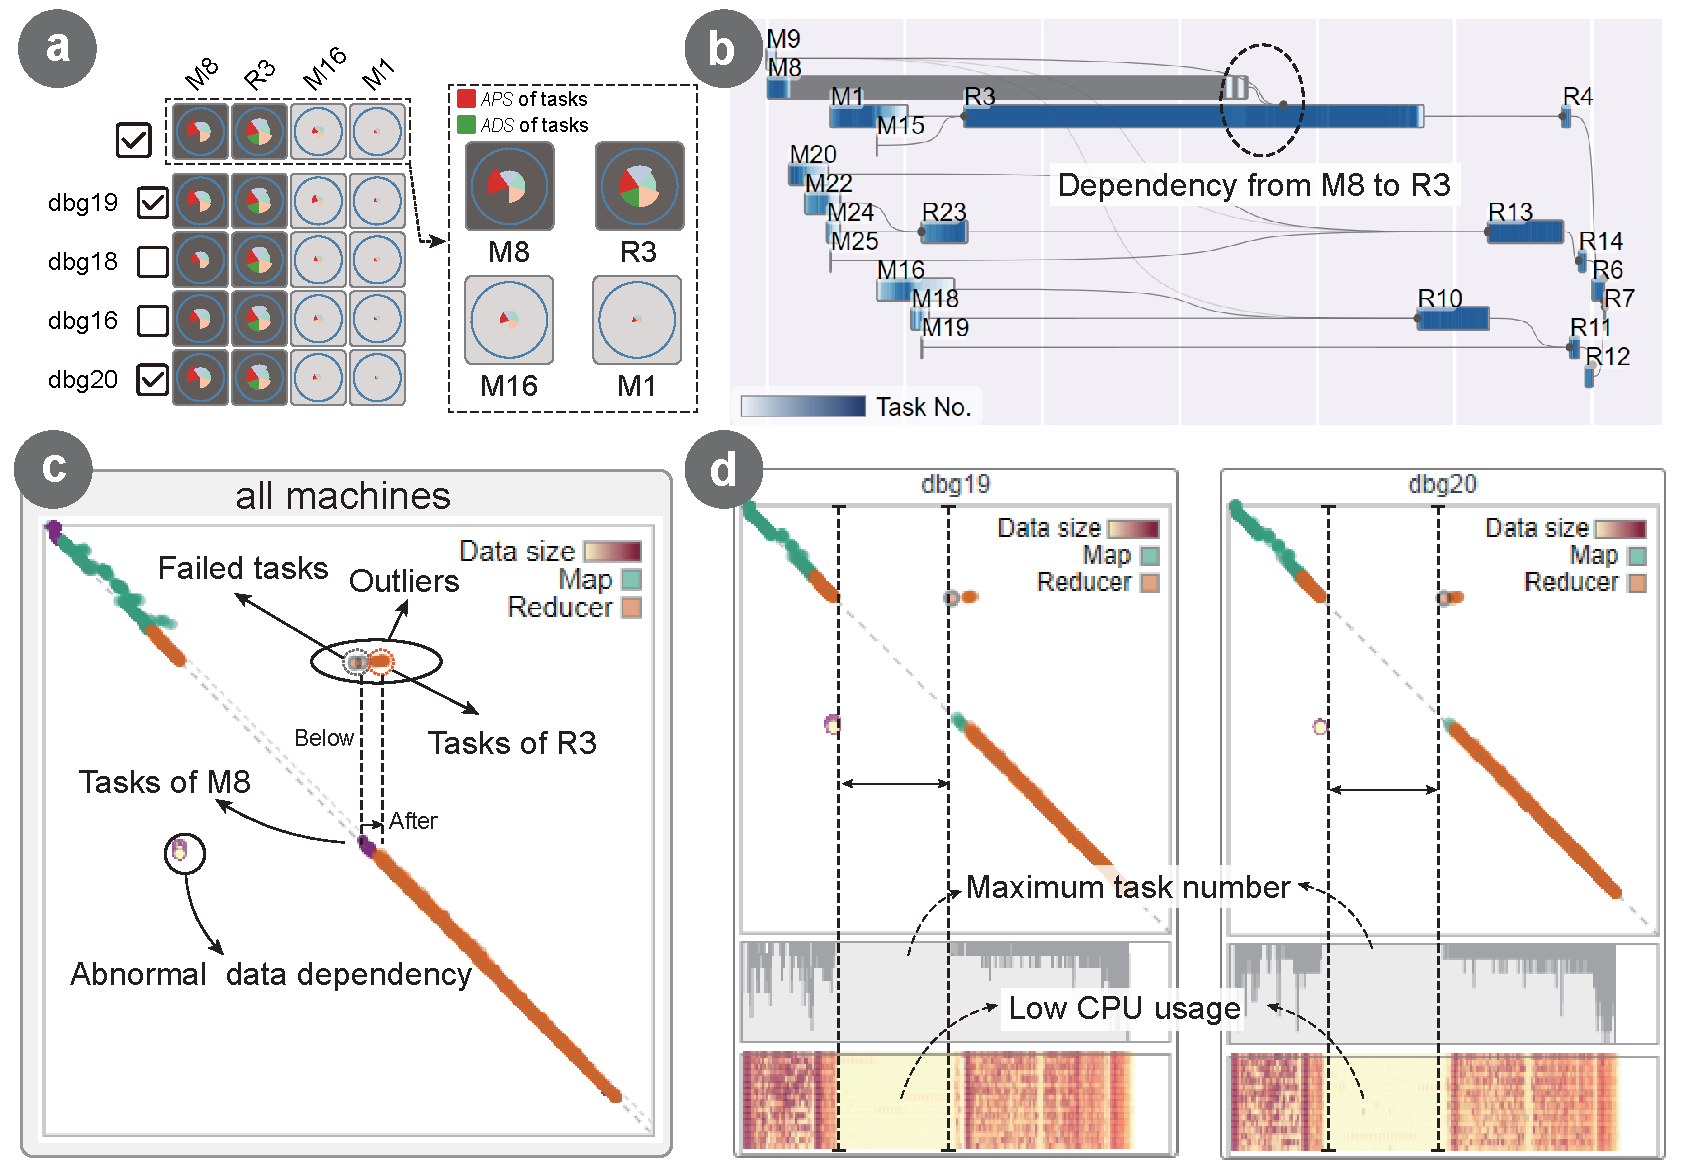
\includegraphics[width=0.46\textwidth]{figures/case_study/CaseStudy2SDS.pdf}  
	\vspace{-3mm}
	\caption{\qevis{} identifies system problem (task deadlock)} 
	\label{fig:casestudy2}
	\vspace{-5mm}
\end{figure}

\stitle{Step 1: observe abnormal jobs via \vtitle{performance matrix}}
As shown by the \textit{performance matrix} in \autoref{fig:casestudy2}(a), the anomaly scores of jobs R3 and M8 are significantly larger than the other jobs, especially the abnormal duration scores (i.e., red sectors). 
Moreover, the green sector (i.e., abnormal parallelism score) of job R3 is also very large.
Since job R3 is the downstream job of M8 as shown in the \textit{job view} in \autoref{fig:casestudy2}(b), 
we conjecture that there is a causal relation between the abnormal behaviors of jobs M8 and R3.


\stitle{Step 2: reveal abnormal data dependency via \vtitle{task view}}
We next perform fine-grained exploration on the tasks via the \vtitle{task view}.
There are several \textbf{outliers}, as highlighted in \autoref{fig:casestudy2}(c).
These outlier tasks can be classified into two categories: (i) failed tasks (the gray points), and (ii) long running tasks (highlighted in orange color).
Interestingly, several tasks of map job M8 are executed immediately after these failed tasks, and then the orange colored tasks of reducer job R3 are executed.
Visually, we can see there are several purple points (i.e., the tasks of job M8) vertically located below the gray points (i.e., failed tasks) and the orange points (i.e., tasks of job R3) are horizontally located after the purple points.
Thus, we confirm that there are abnormal data dependencies among the tasks of jobs M8 and R3, shown as the data dependency points in the left-bottom part of \autoref{fig:casestudy2}(c).


\stitle{Step 3: reason about the failed tasks via \vtitle{profiling view}}
As the \vtitle{profiling view} of the machine is aligned with \vtitle{task view} by time, 
we observe that both dbg19 and dbg20 run the maximum number of tasks during the execution period of these failed tasks, see the range between the two vertical dashed lines for dbg 19 and dbg20 in \autoref{fig:casestudy2}(d). 
However, the CPU utilization of two machines is very low in this period. 
This suggests that the containers of the two machines are fully occupied but no work is done, and thus there is a task deadlock.
In particular, the resource scheduler YARN assigns all containers of dbg19 and dbg20 to the tasks of job R3, and these tasks are waiting for the input data from the upstream tasks of job M8. But the upstream tasks cannot be executed as there are no idle containers, and thus the tasks of jobs M8 and R3 form a circular waiting.
The deadlock is resolved after killing several tasks of job R3, as depicted by the gray colored failed tasks in \autoref{fig:casestudy2}(c).

\qm{
	\stitle{Discussion} 
%	The deadlock appears when the computing resource is limited and too much containers are allocated by source manager(e.g., Yarn). \qevis{} can help analysts identify the deadlock cases with following features: by employing task level visualization with dependencies and properly aligning the timing information of tasks and system profiling.
%Deadlocks occur when computing resources are scarce and an excessive number of containers are allocated by the resource manager (e.g., Yarn). \qevis{} assist analysts to identify deadlock cases through the following features: task-level visualization incorporating dependencies and accurate alignment of timing information from tasks and system profiling. These capabilities enable analysts to gain insights into deadlock situations effectively.
%Deadlocks occur when computing resources are scarce and an excessive number of containers are allocated by the resource manager (e.g., Yarn). \qevis{} assist analysts to identify deadlock cases through the following features: task-level visualization incorporating dependencies and accurate alignment of timing information from tasks and system profiling. These capabilities enable analysts to gain insights into deadlock situations effectively.
%V1
%Deadlocks occur when there's a shortage of computing resources and the resource manager (e.g., Yarn) over-allocates containers. \qevis{} brings following features to address such scenarios: it represents task distribution, enabling users to swiftly identify critical tasks; it displays dependencies that indicate logical relationships among tasks; and it aligns system profiling with execution patterns to illustrate the interplay between resources and execution. The conventional approaches may struggle to manage this situation due to their lack of task oriented visaulization (both task and dependency) and task-system profiling alignment.
%V2
Deadlocks occur when there is a shortage of computing resources and suboptimal task scheduling by resource managers (e.g., Yarn). \qevis{} addresses this by offering following key features: task distribution for quick identification of critical tasks, dependency visualization for understanding logical task relationships and alignment of execution patterns with system profiling to show the interplay between resources and execution. The conventional approaches may struggle to manage this situation due to their lack of task oriented visualization (both task and dependency) and task-system profiling alignment.
}
\subsubsection{Identifying data problem}
We next analyze a query that runs daily for sales analysis, which takes 1200 seconds and is longer than before. 

\begin{figure}[t]
	\centering
	\small
	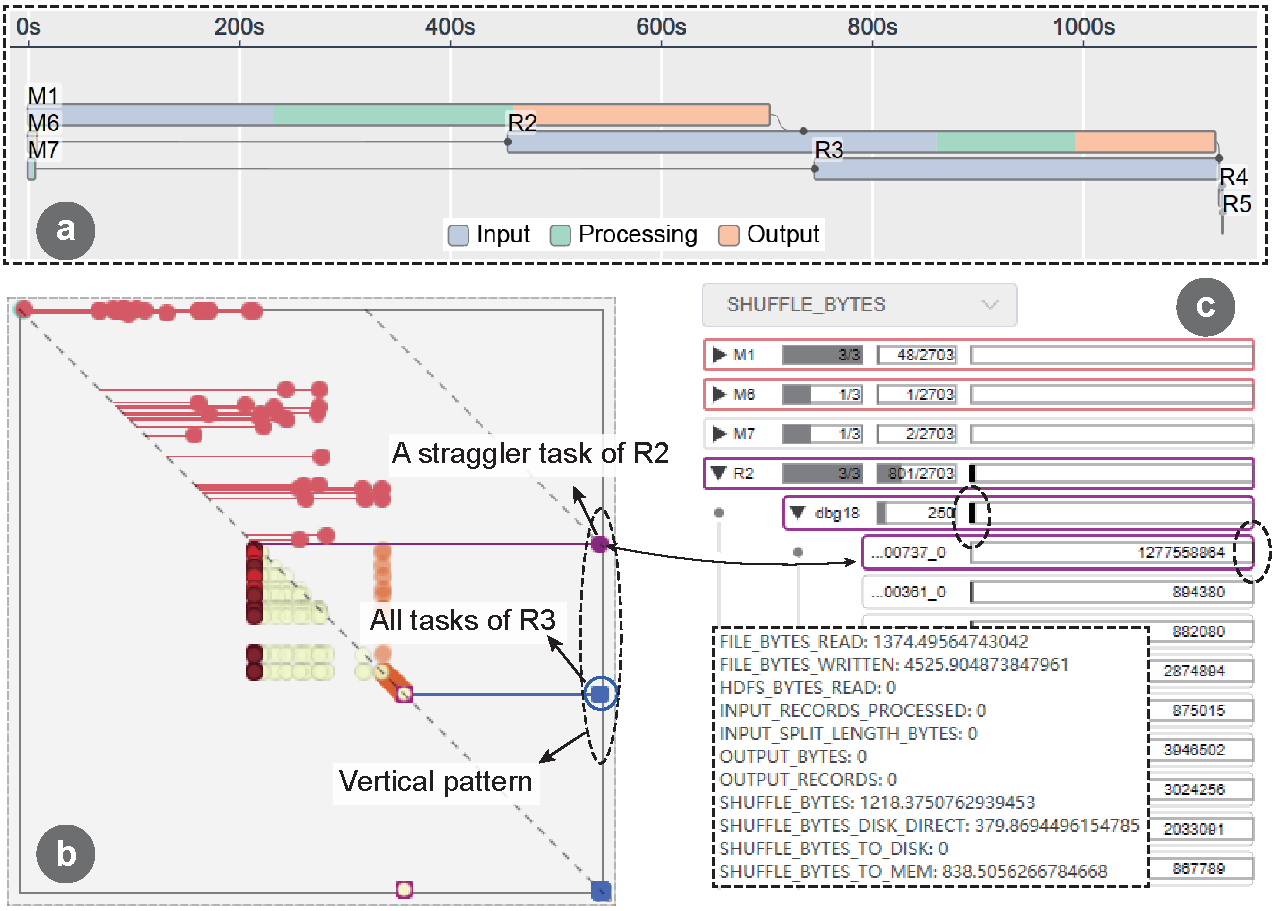
\includegraphics[width=0.46\textwidth]{figures/case_study/CaseStudy3SDS.pdf}
	\vspace{-2mm}
	\caption{\qevis{} detects data skew}
	\label{fig:casestudy3}
	\vspace{-5mm}
\end{figure}


\stitle{Step 1: identify performance bottleneck via \textit{job view}}
We inspect its \vtitle{job view} in \autoref{fig:casestudy3}(a) and observe that the input phase dominates the running time of job R3.
To find the reason for the long input time in job R3, we examine all its tasks via \vtitle{task view} in \autoref{fig:casestudy3}(b).


\stitle{Step 2: locate the straggler task via \textit{task view}}
We find that (i) all tasks of job R3 are concentrated in a small region, and (ii) there is a straggler task of job R2, which are highlighted in blue and purple circles in \autoref{fig:casestudy3}(b), respectively.
Moreover, there is a \textbf{vertical} execution pattern among the tasks of job R3 and the straggler task of job R2,
see the dashed eclipse, which suggests that the downstream tasks (of job R3) are waiting for the upstream task (of job R2).
%We next analyze the straggle task of job R2 via \vtitle{entity list}.

\stitle{Step 3: reason about the straggler task via \vtitle{entity list}}
By clicking the straggler task of job R2 in the \vtitle{task view}, the row of this task is automatically located and highlighted with a purple boundary in \autoref{fig:casestudy3}(c). 
We analyze its long running time by checking its processed data size, i.e., switching to ``SHUFFLE$\_$BYTES'' in the dropdown menu.
Surprisingly, the processed data volume of this straggler task is almost 1000 times of the other tasks in job R2, which indicates a severe data skew among the tasks.
Thus, the above unusually long running query is caused by data skew problem.

\qm{
	\stitle{Discussion} 
%	V1
%	In this case, multiple tasks exhibit abnormal execution behavior, but only one task, which suffers from data skewness, serves as the primary bottleneck for the entire execution process. Accurately identifying this specific bottleneck task necessitates the visualization of both tasks and their dependencies. This crucial visualization capability is provided exclusively by \qevis{}.
This case study highlights a scenario where a single task, experiencing data skewness, acts as the primary bottleneck in the execution process. Although multiple tasks exhibit abnormal execution behavior, correctly pinpointing this specific task is vital. This requires an intricate visualization of tasks along with their dependencies, a feature uniquely offered by \qevis{}.
}

%Through $\qevis$, we can conclude , then experienced engineers will try to alleviate it by re-configure the maximum number of task in Apache \hive{}. 

%\EVA{Can we show the optimization strategy?}



%\subsection{Case study} \label{sec:case}

%$\qevis{}$ has been deployed in the production environment of Huawei Cloud and is widely used by software engineers.
$\qevis{}$ has been deployed in the production environment and is widely used by software engineers.
Usually, our users are interested in queries that run longer than expected because they degrade system throughput. 
In this section, we demonstrate the effectiveness of \qevis{} via three use cases \qm{about slow query} in production, which identifies hardware, system and data problems during query execution, respectively.


\subsubsection{Identifying hardware problem} \label{sec:systemproblem}
\autoref{fig:teaser} shows how \qevis{} visualizes a long running query (i.e., 623 seconds) from a business intelligence application and we analyze it as follows.

\stitle{Step 1: investigate the performance bottleneck via \textit{job view}}
The \textit{job view} of the query is shown in \autoref{fig:teaser}(b).
Visually, job M1 has a very long running time.
More importantly, there is a large gray region in job M1, which means that the number of running tasks is 0 in this region according to the design of job rectangle in \autoref{sec:job}.
Thus, job M1 is the cause of long execution.


\stitle{Step 2: inspect job M1's task execution pattern via \textit{task view}}
To find the reasons that cause the gray region for job M1 in the \textit{job view}, we analyze the tasks of job M1 via the \textit{task view}.
When hovering the mouse on the job rectangle of M1, its associated tasks are highlighted with purple color in the \textit{task view}, see \autoref{fig:teaser}(d). 
We observe that the tasks of job M1 form two groups (i.e., \textbf{multi-cluster} pattern) that are far away from each other, as illustrated by the two dashed ellipses in \autoref{fig:teaser}(d). 
As discussed in \autoref{sec:task}, the multi-cluster pattern suggests that the tasks of job M1 are not executed properly due to machine problems.

\stitle{Step 3: locate the problematic machine via \textit{entity list}}
We know that the long running query is caused by machine problems but it is difficult to pinpoint the problematic machines as the production cluster is large.
Fortunately, \qevis{} provides the \textit{entity list} to map tasks to their executing machines.
By checking the \textit{entity list}, as illustrated by the rows with purple stroke in \autoref{fig:teaser}(e1), 
we observe that the tasks of job M1 in the right-bottom corner are executed on machine dbg18
%~\footnote{We anonymize the machine identifiers as required by our industry partner.}.
Then, we take a closer look at the tasks executed on dbg18, see \autoref{fig:teaser}(d1).
Compared with the other machines (e.g., dbg16, dbg19, dbg20), the number of tasks executed by dbg18 is quite small,
which suggests that the resource scheduler YARN allocates a small number of tasks to dbg18. 
This confirms that dbg18 is the problematic machine and YARN is aware of this fact during the query execution progress.
%With the conclusion above, we contact the infrastructure team and they confirm with us that the hard disk of dbg18 incurs errors.

Similar analyzing steps are also applied to job M24, which is another long running job in the query. 
We find that the long running time of job M24 is caused by a few straggling tasks on dbg19.
By investigating them, we find that dbg19 has high CPU utilization, see the red regions of the CPU usage heatmap in \autoref{fig:teaser}(f). 
We omit its analyzed steps as they are similar to the steps for job M1. 

To sum up, hardware problems cause the long running query. 
To verify, we remove dbg18 and dbg19, and re-run the query. The running time becomes 200 seconds.
\autoref{fig:teaser}(b1) shows the new \textit{job view}, where the running time of jobs M1 and M24 are much shorter than before.

\qm{
\stitle{Discussion}
%In this case study, the task cross-view linage and task level visualization analysis plays an important role in facilitate the execution exploration. Through the linkage among \vtitle{job view} and \vtitle{task view}, we quickly find the abnormal tasks (the group of late executed tasks) and then find these tasks are executed on a problematic machine which run very few tasks. 
%In this case study, the long execution of query is caused by multiple hardware problem, which is commonly appeared in real applications. The task level visualization of \qevis{} is key to facilitate exploration in this case. It allows users to quickly identify the abnormal tasks. Then we find their commonness through the cross-view linkage (\vtitle{task view} and \vtitle{entity list}), which is that all of these machines are executed on dbg18. Then we use \vtitle{task view} of dbg18 to confirm that the machine is suffering from hardware problem. 
%In this case study, the prolonged query execution is attributed to several hardware issues, a common occurrence in real-world applications. The task-level visualization provided by \qevis{} plays a crucial role in aiding exploration in this particular case. It enables users to promptly identify abnormal tasks. Through cross-view linkage, specifically between the task view and entity list, we determine a common factor: all these tasks are executed on dbg18. Further utilizing the task view of dbg18, we confirm that the machine is indeed experiencing a hardware problem.
%In this case study, the query execution suffers from multiple hardware issues. The \vtitle{task view} of all tasks plays a crucial role in aiding exploration by enabling users to promptly identify the abnormal tasks. The \vtitle{task view} of dbg18 further shows that the machine dbg18 which executes the abnormal tasks is suffering from a hardware problem.
%
%The \vtitle{task view} offered by \qevis{} plays a crucial role in aiding exploration by enabling users to promptly identify the abnormal tasks.  Then we confirm these tasks are executed on the same machine dbg18 through the linkage between \vtitle{task view} and \vtitle{entity list}, and inspect taht this machine is indeed experiencing a hardware problem. 
In this case study, the query execution suffers from multiple hardware issues. The \vtitle{task view} of all tasks plays a crucial role by quickly identifying abnormal tasks. Furthermore, the \vtitle{task view} of dbg18 further shows that the machine dbg18 which executes the abnormal tasks is suffering from a hardware problem. This scenario demonstrates that the visual pattern of tasks is helpful in diagnosing these issues efficiently.
}

\subsubsection{Identifying system problem}
We analyze a query that generates app downloads report for market analysis in this case.
\begin{figure}
	\centering
	\small
	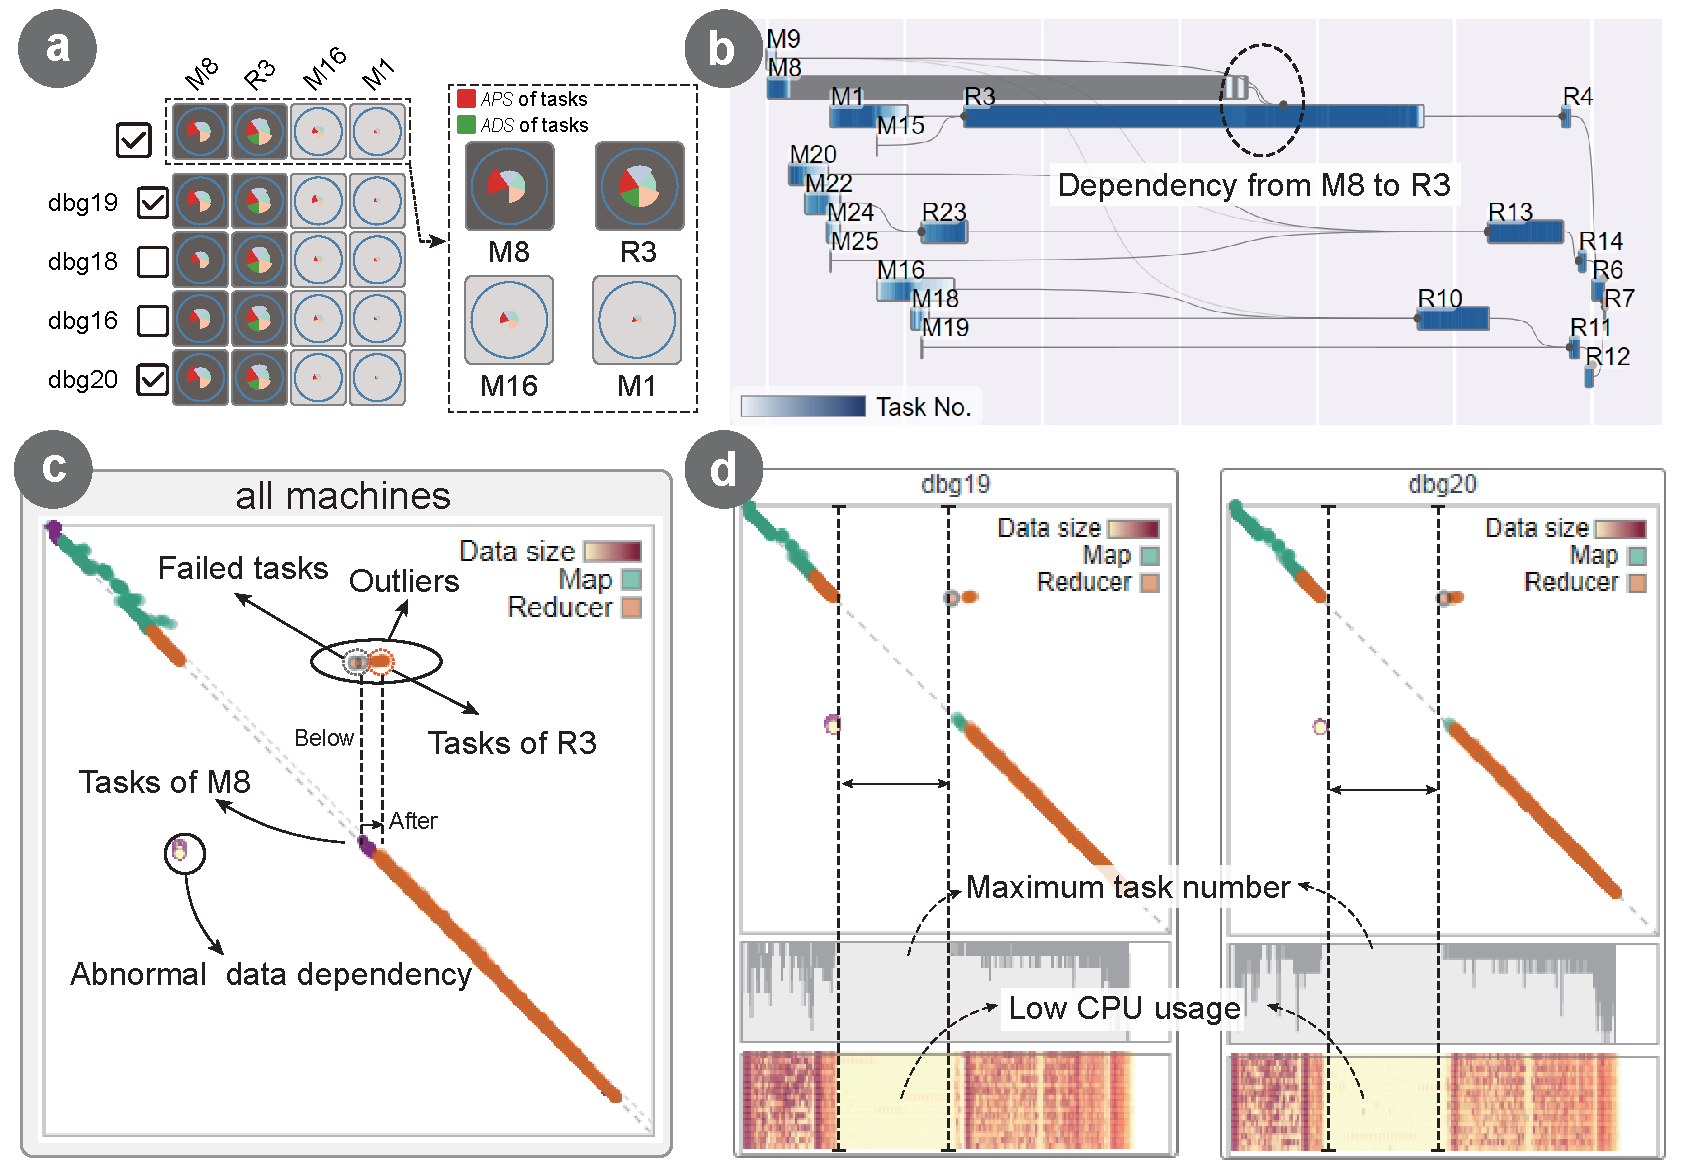
\includegraphics[width=0.46\textwidth]{figures/case_study/CaseStudy2SDS.pdf}  
	\vspace{-3mm}
	\caption{\qevis{} identifies system problem (task deadlock)} 
	\label{fig:casestudy2}
	\vspace{-5mm}
\end{figure}

\stitle{Step 1: observe abnormal jobs via \vtitle{performance matrix}}
As shown by the \textit{performance matrix} in \autoref{fig:casestudy2}(a), the anomaly scores of jobs R3 and M8 are significantly larger than the other jobs, especially the abnormal duration scores (i.e., red sectors). 
Moreover, the green sector (i.e., abnormal parallelism score) of job R3 is also very large.
Since job R3 is the downstream job of M8 as shown in the \textit{job view} in \autoref{fig:casestudy2}(b), 
we conjecture that there is a causal relation between the abnormal behaviors of jobs M8 and R3.


\stitle{Step 2: reveal abnormal data dependency via \vtitle{task view}}
We next perform fine-grained exploration on the tasks via the \vtitle{task view}.
There are several \textbf{outliers}, as highlighted in \autoref{fig:casestudy2}(c).
These outlier tasks can be classified into two categories: (i) failed tasks (the gray points), and (ii) long running tasks (highlighted in orange color).
Interestingly, several tasks of map job M8 are executed immediately after these failed tasks, and then the orange colored tasks of reducer job R3 are executed.
Visually, we can see there are several purple points (i.e., the tasks of job M8) vertically located below the gray points (i.e., failed tasks) and the orange points (i.e., tasks of job R3) are horizontally located after the purple points.
Thus, we confirm that there are abnormal data dependencies among the tasks of jobs M8 and R3, shown as the data dependency points in the left-bottom part of \autoref{fig:casestudy2}(c).


\stitle{Step 3: reason about the failed tasks via \vtitle{profiling view}}
As the \vtitle{profiling view} of the machine is aligned with \vtitle{task view} by time, 
we observe that both dbg19 and dbg20 run the maximum number of tasks during the execution period of these failed tasks, see the range between the two vertical dashed lines for dbg 19 and dbg20 in \autoref{fig:casestudy2}(d). 
However, the CPU utilization of two machines is very low in this period. 
This suggests that the containers of the two machines are fully occupied but no work is done, and thus there is a task deadlock.
In particular, the resource scheduler YARN assigns all containers of dbg19 and dbg20 to the tasks of job R3, and these tasks are waiting for the input data from the upstream tasks of job M8. But the upstream tasks cannot be executed as there are no idle containers, and thus the tasks of jobs M8 and R3 form a circular waiting.
The deadlock is resolved after killing several tasks of job R3, as depicted by the gray colored failed tasks in \autoref{fig:casestudy2}(c).

\qm{
	\stitle{Discussion} 
%	The deadlock appears when the computing resource is limited and too much containers are allocated by source manager(e.g., Yarn). \qevis{} can help analysts identify the deadlock cases with following features: by employing task level visualization with dependencies and properly aligning the timing information of tasks and system profiling.
%Deadlocks occur when computing resources are scarce and an excessive number of containers are allocated by the resource manager (e.g., Yarn). \qevis{} assist analysts to identify deadlock cases through the following features: task-level visualization incorporating dependencies and accurate alignment of timing information from tasks and system profiling. These capabilities enable analysts to gain insights into deadlock situations effectively.
%Deadlocks occur when computing resources are scarce and an excessive number of containers are allocated by the resource manager (e.g., Yarn). \qevis{} assist analysts to identify deadlock cases through the following features: task-level visualization incorporating dependencies and accurate alignment of timing information from tasks and system profiling. These capabilities enable analysts to gain insights into deadlock situations effectively.
%V1
%Deadlocks occur when there's a shortage of computing resources and the resource manager (e.g., Yarn) over-allocates containers. \qevis{} brings following features to address such scenarios: it represents task distribution, enabling users to swiftly identify critical tasks; it displays dependencies that indicate logical relationships among tasks; and it aligns system profiling with execution patterns to illustrate the interplay between resources and execution. The conventional approaches may struggle to manage this situation due to their lack of task oriented visaulization (both task and dependency) and task-system profiling alignment.
%V2
Deadlocks occur when there is a shortage of computing resources and suboptimal task scheduling by resource managers (e.g., Yarn). \qevis{} addresses this by offering following key features: task distribution for quick identification of critical tasks, dependency visualization for understanding logical task relationships and alignment of execution patterns with system profiling to show the interplay between resources and execution. The conventional approaches may struggle to manage this situation due to their lack of task oriented visualization (both task and dependency) and task-system profiling alignment.
}
\subsubsection{Identifying data problem}
We next analyze a query that runs daily for sales analysis, which takes 1200 seconds and is longer than before. 

\begin{figure}[t]
	\centering
	\small
	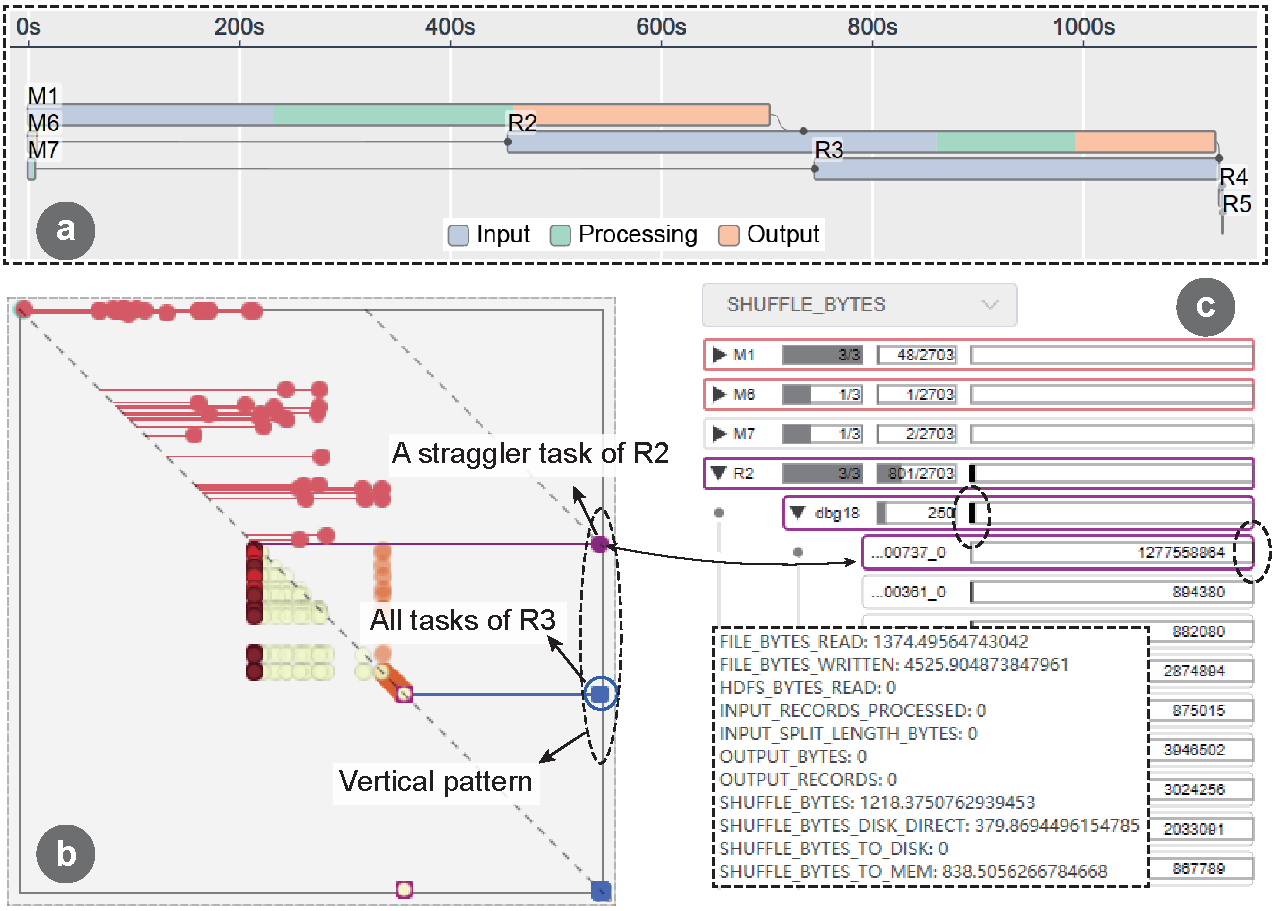
\includegraphics[width=0.46\textwidth]{figures/case_study/CaseStudy3SDS.pdf}
	\vspace{-2mm}
	\caption{\qevis{} detects data skew}
	\label{fig:casestudy3}
	\vspace{-5mm}
\end{figure}


\stitle{Step 1: identify performance bottleneck via \textit{job view}}
We inspect its \vtitle{job view} in \autoref{fig:casestudy3}(a) and observe that the input phase dominates the running time of job R3.
To find the reason for the long input time in job R3, we examine all its tasks via \vtitle{task view} in \autoref{fig:casestudy3}(b).


\stitle{Step 2: locate the straggler task via \textit{task view}}
We find that (i) all tasks of job R3 are concentrated in a small region, and (ii) there is a straggler task of job R2, which are highlighted in blue and purple circles in \autoref{fig:casestudy3}(b), respectively.
Moreover, there is a \textbf{vertical} execution pattern among the tasks of job R3 and the straggler task of job R2,
see the dashed eclipse, which suggests that the downstream tasks (of job R3) are waiting for the upstream task (of job R2).
%We next analyze the straggle task of job R2 via \vtitle{entity list}.

\stitle{Step 3: reason about the straggler task via \vtitle{entity list}}
By clicking the straggler task of job R2 in the \vtitle{task view}, the row of this task is automatically located and highlighted with a purple boundary in \autoref{fig:casestudy3}(c). 
We analyze its long running time by checking its processed data size, i.e., switching to ``SHUFFLE$\_$BYTES'' in the dropdown menu.
Surprisingly, the processed data volume of this straggler task is almost 1000 times of the other tasks in job R2, which indicates a severe data skew among the tasks.
Thus, the above unusually long running query is caused by data skew problem.

\qm{
	\stitle{Discussion} 
%	V1
%	In this case, multiple tasks exhibit abnormal execution behavior, but only one task, which suffers from data skewness, serves as the primary bottleneck for the entire execution process. Accurately identifying this specific bottleneck task necessitates the visualization of both tasks and their dependencies. This crucial visualization capability is provided exclusively by \qevis{}.
This case study highlights a scenario where a single task, experiencing data skewness, acts as the primary bottleneck in the execution process. Although multiple tasks exhibit abnormal execution behavior, correctly pinpointing this specific task is vital. This requires an intricate visualization of tasks along with their dependencies, a feature uniquely offered by \qevis{}.
}

%Through $\qevis$, we can conclude , then experienced engineers will try to alleviate it by re-configure the maximum number of task in Apache \hive{}. 

%\EVA{Can we show the optimization strategy?}



%\subsection{Case study} \label{sec:case}

%$\qevis{}$ has been deployed in the production environment of Huawei Cloud and is widely used by software engineers.
$\qevis{}$ has been deployed in the production environment and is widely used by software engineers.
Usually, our users are interested in queries that run longer than expected because they degrade system throughput. 
In this section, we demonstrate the effectiveness of \qevis{} via three use cases \qm{about slow query} in production, which identifies hardware, system and data problems during query execution, respectively.


\subsubsection{Identifying hardware problem} \label{sec:systemproblem}
\autoref{fig:teaser} shows how \qevis{} visualizes a long running query (i.e., 623 seconds) from a business intelligence application and we analyze it as follows.

\stitle{Step 1: investigate the performance bottleneck via \textit{job view}}
The \textit{job view} of the query is shown in \autoref{fig:teaser}(b).
Visually, job M1 has a very long running time.
More importantly, there is a large gray region in job M1, which means that the number of running tasks is 0 in this region according to the design of job rectangle in \autoref{sec:job}.
Thus, job M1 is the cause of long execution.


\stitle{Step 2: inspect job M1's task execution pattern via \textit{task view}}
To find the reasons that cause the gray region for job M1 in the \textit{job view}, we analyze the tasks of job M1 via the \textit{task view}.
When hovering the mouse on the job rectangle of M1, its associated tasks are highlighted with purple color in the \textit{task view}, see \autoref{fig:teaser}(d). 
We observe that the tasks of job M1 form two groups (i.e., \textbf{multi-cluster} pattern) that are far away from each other, as illustrated by the two dashed ellipses in \autoref{fig:teaser}(d). 
As discussed in \autoref{sec:task}, the multi-cluster pattern suggests that the tasks of job M1 are not executed properly due to machine problems.

\stitle{Step 3: locate the problematic machine via \textit{entity list}}
We know that the long running query is caused by machine problems but it is difficult to pinpoint the problematic machines as the production cluster is large.
Fortunately, \qevis{} provides the \textit{entity list} to map tasks to their executing machines.
By checking the \textit{entity list}, as illustrated by the rows with purple stroke in \autoref{fig:teaser}(e1), 
we observe that the tasks of job M1 in the right-bottom corner are executed on machine dbg18
%~\footnote{We anonymize the machine identifiers as required by our industry partner.}.
Then, we take a closer look at the tasks executed on dbg18, see \autoref{fig:teaser}(d1).
Compared with the other machines (e.g., dbg16, dbg19, dbg20), the number of tasks executed by dbg18 is quite small,
which suggests that the resource scheduler YARN allocates a small number of tasks to dbg18. 
This confirms that dbg18 is the problematic machine and YARN is aware of this fact during the query execution progress.
%With the conclusion above, we contact the infrastructure team and they confirm with us that the hard disk of dbg18 incurs errors.

Similar analyzing steps are also applied to job M24, which is another long running job in the query. 
We find that the long running time of job M24 is caused by a few straggling tasks on dbg19.
By investigating them, we find that dbg19 has high CPU utilization, see the red regions of the CPU usage heatmap in \autoref{fig:teaser}(f). 
We omit its analyzed steps as they are similar to the steps for job M1. 

To sum up, hardware problems cause the long running query. 
To verify, we remove dbg18 and dbg19, and re-run the query. The running time becomes 200 seconds.
\autoref{fig:teaser}(b1) shows the new \textit{job view}, where the running time of jobs M1 and M24 are much shorter than before.

\qm{
\stitle{Discussion}
%In this case study, the task cross-view linage and task level visualization analysis plays an important role in facilitate the execution exploration. Through the linkage among \vtitle{job view} and \vtitle{task view}, we quickly find the abnormal tasks (the group of late executed tasks) and then find these tasks are executed on a problematic machine which run very few tasks. 
%In this case study, the long execution of query is caused by multiple hardware problem, which is commonly appeared in real applications. The task level visualization of \qevis{} is key to facilitate exploration in this case. It allows users to quickly identify the abnormal tasks. Then we find their commonness through the cross-view linkage (\vtitle{task view} and \vtitle{entity list}), which is that all of these machines are executed on dbg18. Then we use \vtitle{task view} of dbg18 to confirm that the machine is suffering from hardware problem. 
%In this case study, the prolonged query execution is attributed to several hardware issues, a common occurrence in real-world applications. The task-level visualization provided by \qevis{} plays a crucial role in aiding exploration in this particular case. It enables users to promptly identify abnormal tasks. Through cross-view linkage, specifically between the task view and entity list, we determine a common factor: all these tasks are executed on dbg18. Further utilizing the task view of dbg18, we confirm that the machine is indeed experiencing a hardware problem.
%In this case study, the query execution suffers from multiple hardware issues. The \vtitle{task view} of all tasks plays a crucial role in aiding exploration by enabling users to promptly identify the abnormal tasks. The \vtitle{task view} of dbg18 further shows that the machine dbg18 which executes the abnormal tasks is suffering from a hardware problem.
%
%The \vtitle{task view} offered by \qevis{} plays a crucial role in aiding exploration by enabling users to promptly identify the abnormal tasks.  Then we confirm these tasks are executed on the same machine dbg18 through the linkage between \vtitle{task view} and \vtitle{entity list}, and inspect taht this machine is indeed experiencing a hardware problem. 
In this case study, the query execution suffers from multiple hardware issues. The \vtitle{task view} of all tasks plays a crucial role by quickly identifying abnormal tasks. Furthermore, the \vtitle{task view} of dbg18 further shows that the machine dbg18 which executes the abnormal tasks is suffering from a hardware problem. This scenario demonstrates that the visual pattern of tasks is helpful in diagnosing these issues efficiently.
}

\subsubsection{Identifying system problem}
We analyze a query that generates app downloads report for market analysis in this case.
\begin{figure}
	\centering
	\small
	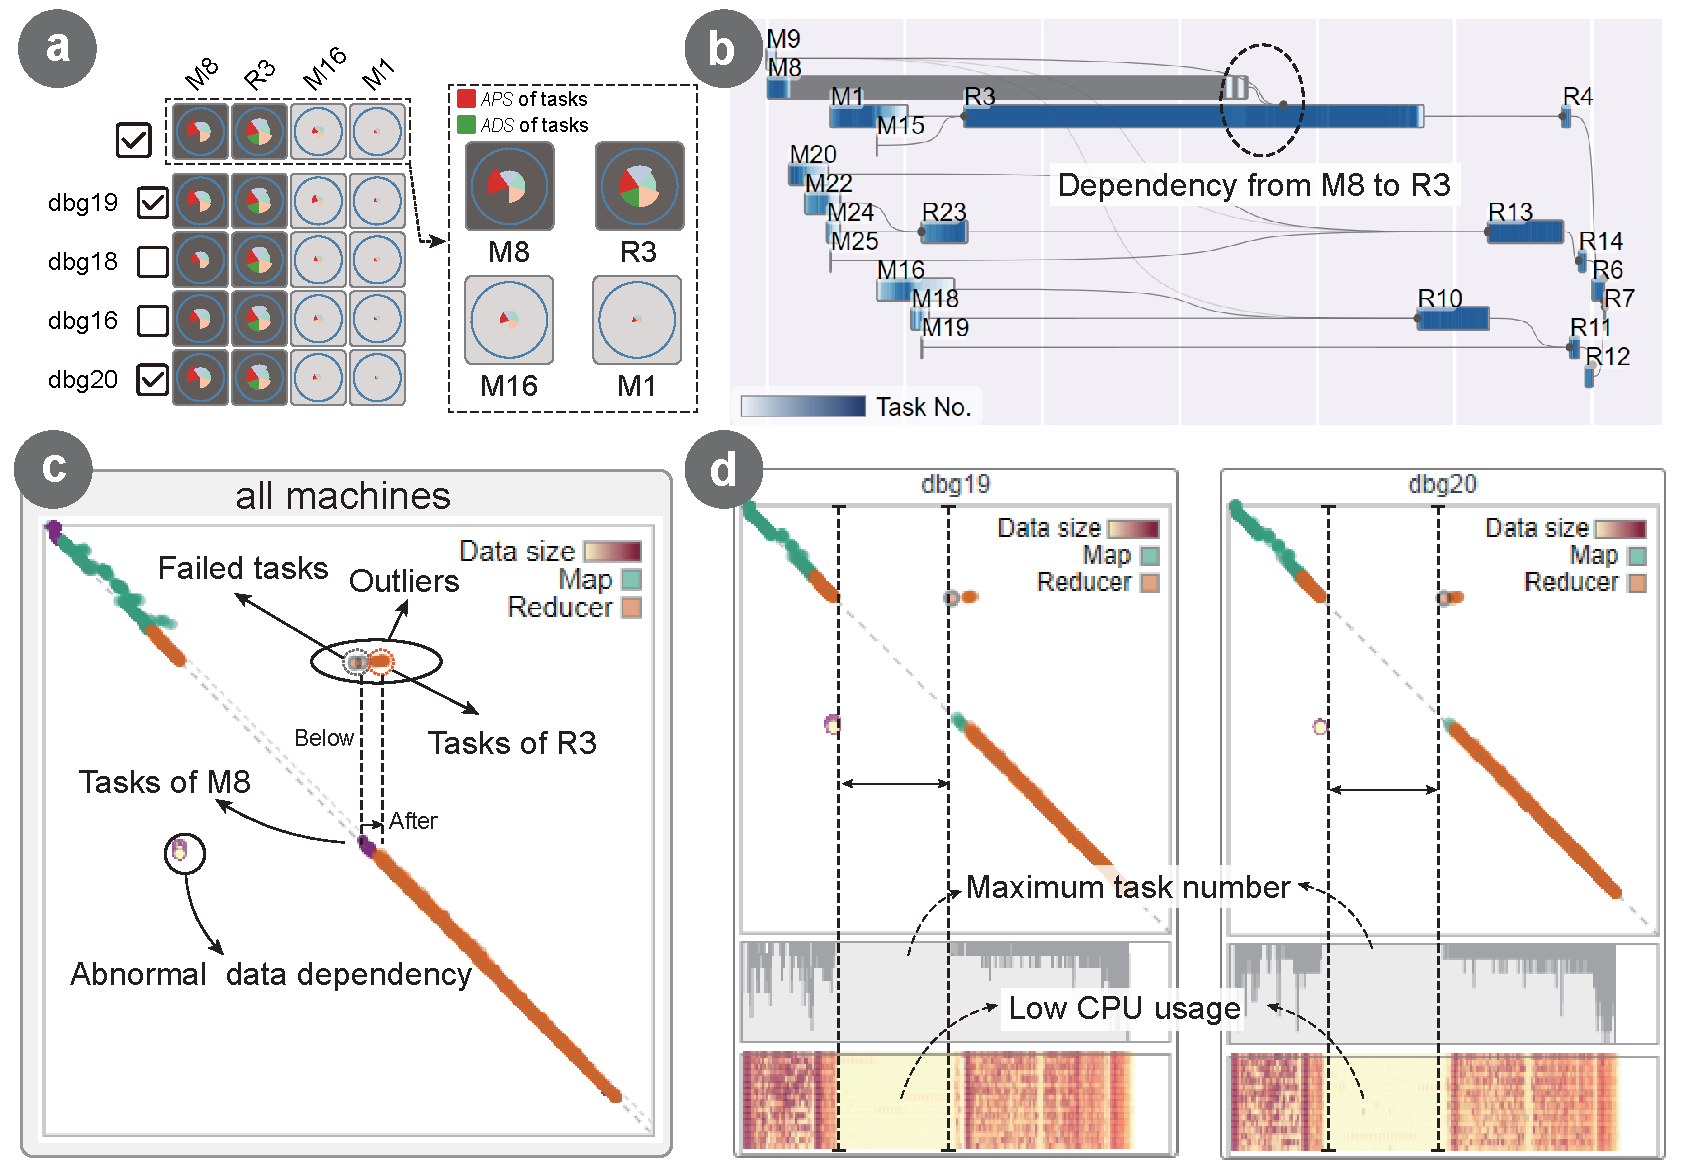
\includegraphics[width=0.46\textwidth]{figures/case_study/CaseStudy2SDS.pdf}  
	\vspace{-3mm}
	\caption{\qevis{} identifies system problem (task deadlock)} 
	\label{fig:casestudy2}
	\vspace{-5mm}
\end{figure}

\stitle{Step 1: observe abnormal jobs via \vtitle{performance matrix}}
As shown by the \textit{performance matrix} in \autoref{fig:casestudy2}(a), the anomaly scores of jobs R3 and M8 are significantly larger than the other jobs, especially the abnormal duration scores (i.e., red sectors). 
Moreover, the green sector (i.e., abnormal parallelism score) of job R3 is also very large.
Since job R3 is the downstream job of M8 as shown in the \textit{job view} in \autoref{fig:casestudy2}(b), 
we conjecture that there is a causal relation between the abnormal behaviors of jobs M8 and R3.


\stitle{Step 2: reveal abnormal data dependency via \vtitle{task view}}
We next perform fine-grained exploration on the tasks via the \vtitle{task view}.
There are several \textbf{outliers}, as highlighted in \autoref{fig:casestudy2}(c).
These outlier tasks can be classified into two categories: (i) failed tasks (the gray points), and (ii) long running tasks (highlighted in orange color).
Interestingly, several tasks of map job M8 are executed immediately after these failed tasks, and then the orange colored tasks of reducer job R3 are executed.
Visually, we can see there are several purple points (i.e., the tasks of job M8) vertically located below the gray points (i.e., failed tasks) and the orange points (i.e., tasks of job R3) are horizontally located after the purple points.
Thus, we confirm that there are abnormal data dependencies among the tasks of jobs M8 and R3, shown as the data dependency points in the left-bottom part of \autoref{fig:casestudy2}(c).


\stitle{Step 3: reason about the failed tasks via \vtitle{profiling view}}
As the \vtitle{profiling view} of the machine is aligned with \vtitle{task view} by time, 
we observe that both dbg19 and dbg20 run the maximum number of tasks during the execution period of these failed tasks, see the range between the two vertical dashed lines for dbg 19 and dbg20 in \autoref{fig:casestudy2}(d). 
However, the CPU utilization of two machines is very low in this period. 
This suggests that the containers of the two machines are fully occupied but no work is done, and thus there is a task deadlock.
In particular, the resource scheduler YARN assigns all containers of dbg19 and dbg20 to the tasks of job R3, and these tasks are waiting for the input data from the upstream tasks of job M8. But the upstream tasks cannot be executed as there are no idle containers, and thus the tasks of jobs M8 and R3 form a circular waiting.
The deadlock is resolved after killing several tasks of job R3, as depicted by the gray colored failed tasks in \autoref{fig:casestudy2}(c).

\qm{
	\stitle{Discussion} 
%	The deadlock appears when the computing resource is limited and too much containers are allocated by source manager(e.g., Yarn). \qevis{} can help analysts identify the deadlock cases with following features: by employing task level visualization with dependencies and properly aligning the timing information of tasks and system profiling.
%Deadlocks occur when computing resources are scarce and an excessive number of containers are allocated by the resource manager (e.g., Yarn). \qevis{} assist analysts to identify deadlock cases through the following features: task-level visualization incorporating dependencies and accurate alignment of timing information from tasks and system profiling. These capabilities enable analysts to gain insights into deadlock situations effectively.
%Deadlocks occur when computing resources are scarce and an excessive number of containers are allocated by the resource manager (e.g., Yarn). \qevis{} assist analysts to identify deadlock cases through the following features: task-level visualization incorporating dependencies and accurate alignment of timing information from tasks and system profiling. These capabilities enable analysts to gain insights into deadlock situations effectively.
%V1
%Deadlocks occur when there's a shortage of computing resources and the resource manager (e.g., Yarn) over-allocates containers. \qevis{} brings following features to address such scenarios: it represents task distribution, enabling users to swiftly identify critical tasks; it displays dependencies that indicate logical relationships among tasks; and it aligns system profiling with execution patterns to illustrate the interplay between resources and execution. The conventional approaches may struggle to manage this situation due to their lack of task oriented visaulization (both task and dependency) and task-system profiling alignment.
%V2
Deadlocks occur when there is a shortage of computing resources and suboptimal task scheduling by resource managers (e.g., Yarn). \qevis{} addresses this by offering following key features: task distribution for quick identification of critical tasks, dependency visualization for understanding logical task relationships and alignment of execution patterns with system profiling to show the interplay between resources and execution. The conventional approaches may struggle to manage this situation due to their lack of task oriented visualization (both task and dependency) and task-system profiling alignment.
}
\subsubsection{Identifying data problem}
We next analyze a query that runs daily for sales analysis, which takes 1200 seconds and is longer than before. 

\begin{figure}[t]
	\centering
	\small
	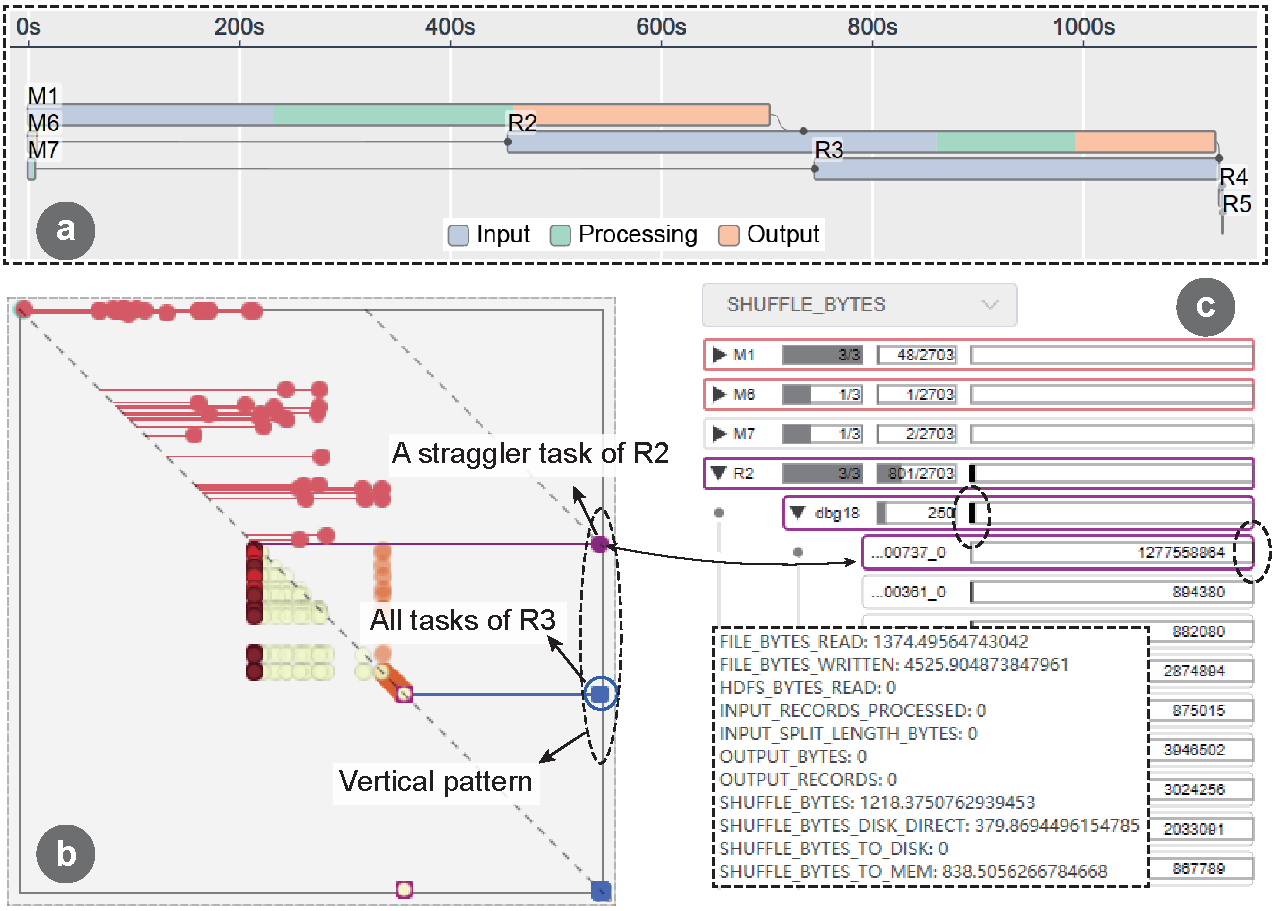
\includegraphics[width=0.46\textwidth]{figures/case_study/CaseStudy3SDS.pdf}
	\vspace{-2mm}
	\caption{\qevis{} detects data skew}
	\label{fig:casestudy3}
	\vspace{-5mm}
\end{figure}


\stitle{Step 1: identify performance bottleneck via \textit{job view}}
We inspect its \vtitle{job view} in \autoref{fig:casestudy3}(a) and observe that the input phase dominates the running time of job R3.
To find the reason for the long input time in job R3, we examine all its tasks via \vtitle{task view} in \autoref{fig:casestudy3}(b).


\stitle{Step 2: locate the straggler task via \textit{task view}}
We find that (i) all tasks of job R3 are concentrated in a small region, and (ii) there is a straggler task of job R2, which are highlighted in blue and purple circles in \autoref{fig:casestudy3}(b), respectively.
Moreover, there is a \textbf{vertical} execution pattern among the tasks of job R3 and the straggler task of job R2,
see the dashed eclipse, which suggests that the downstream tasks (of job R3) are waiting for the upstream task (of job R2).
%We next analyze the straggle task of job R2 via \vtitle{entity list}.

\stitle{Step 3: reason about the straggler task via \vtitle{entity list}}
By clicking the straggler task of job R2 in the \vtitle{task view}, the row of this task is automatically located and highlighted with a purple boundary in \autoref{fig:casestudy3}(c). 
We analyze its long running time by checking its processed data size, i.e., switching to ``SHUFFLE$\_$BYTES'' in the dropdown menu.
Surprisingly, the processed data volume of this straggler task is almost 1000 times of the other tasks in job R2, which indicates a severe data skew among the tasks.
Thus, the above unusually long running query is caused by data skew problem.

\qm{
	\stitle{Discussion} 
%	V1
%	In this case, multiple tasks exhibit abnormal execution behavior, but only one task, which suffers from data skewness, serves as the primary bottleneck for the entire execution process. Accurately identifying this specific bottleneck task necessitates the visualization of both tasks and their dependencies. This crucial visualization capability is provided exclusively by \qevis{}.
This case study highlights a scenario where a single task, experiencing data skewness, acts as the primary bottleneck in the execution process. Although multiple tasks exhibit abnormal execution behavior, correctly pinpointing this specific task is vital. This requires an intricate visualization of tasks along with their dependencies, a feature uniquely offered by \qevis{}.
}

%Through $\qevis$, we can conclude , then experienced engineers will try to alleviate it by re-configure the maximum number of task in Apache \hive{}. 

%\EVA{Can we show the optimization strategy?}



%\subsection{Case study} \label{sec:case}

%$\qevis{}$ has been deployed in the production environment of Huawei Cloud and is widely used by software engineers.
$\qevis{}$ has been deployed in the production environment and is widely used by software engineers.
Usually, our users are interested in queries that run longer than expected because they degrade system throughput. 
In this section, we demonstrate the effectiveness of \qevis{} via three use cases \qm{about slow query} in production, which identifies hardware, system and data problems during query execution, respectively.


\subsubsection{Identifying hardware problem} \label{sec:systemproblem}
\autoref{fig:teaser} shows how \qevis{} visualizes a long running query (i.e., 623 seconds) from a business intelligence application and we analyze it as follows.

\stitle{Step 1: investigate the performance bottleneck via \textit{job view}}
The \textit{job view} of the query is shown in \autoref{fig:teaser}(b).
Visually, job M1 has a very long running time.
More importantly, there is a large gray region in job M1, which means that the number of running tasks is 0 in this region according to the design of job rectangle in \autoref{sec:job}.
Thus, job M1 is the cause of long execution.


\stitle{Step 2: inspect job M1's task execution pattern via \textit{task view}}
To find the reasons that cause the gray region for job M1 in the \textit{job view}, we analyze the tasks of job M1 via the \textit{task view}.
When hovering the mouse on the job rectangle of M1, its associated tasks are highlighted with purple color in the \textit{task view}, see \autoref{fig:teaser}(d). 
We observe that the tasks of job M1 form two groups (i.e., \textbf{multi-cluster} pattern) that are far away from each other, as illustrated by the two dashed ellipses in \autoref{fig:teaser}(d). 
As discussed in \autoref{sec:task}, the multi-cluster pattern suggests that the tasks of job M1 are not executed properly due to machine problems.

\stitle{Step 3: locate the problematic machine via \textit{entity list}}
We know that the long running query is caused by machine problems but it is difficult to pinpoint the problematic machines as the production cluster is large.
Fortunately, \qevis{} provides the \textit{entity list} to map tasks to their executing machines.
By checking the \textit{entity list}, as illustrated by the rows with purple stroke in \autoref{fig:teaser}(e1), 
we observe that the tasks of job M1 in the right-bottom corner are executed on machine dbg18
%~\footnote{We anonymize the machine identifiers as required by our industry partner.}.
Then, we take a closer look at the tasks executed on dbg18, see \autoref{fig:teaser}(d1).
Compared with the other machines (e.g., dbg16, dbg19, dbg20), the number of tasks executed by dbg18 is quite small,
which suggests that the resource scheduler YARN allocates a small number of tasks to dbg18. 
This confirms that dbg18 is the problematic machine and YARN is aware of this fact during the query execution progress.
%With the conclusion above, we contact the infrastructure team and they confirm with us that the hard disk of dbg18 incurs errors.

Similar analyzing steps are also applied to job M24, which is another long running job in the query. 
We find that the long running time of job M24 is caused by a few straggling tasks on dbg19.
By investigating them, we find that dbg19 has high CPU utilization, see the red regions of the CPU usage heatmap in \autoref{fig:teaser}(f). 
We omit its analyzed steps as they are similar to the steps for job M1. 

To sum up, hardware problems cause the long running query. 
To verify, we remove dbg18 and dbg19, and re-run the query. The running time becomes 200 seconds.
\autoref{fig:teaser}(b1) shows the new \textit{job view}, where the running time of jobs M1 and M24 are much shorter than before.

\qm{
\stitle{Discussion}
%In this case study, the task cross-view linage and task level visualization analysis plays an important role in facilitate the execution exploration. Through the linkage among \vtitle{job view} and \vtitle{task view}, we quickly find the abnormal tasks (the group of late executed tasks) and then find these tasks are executed on a problematic machine which run very few tasks. 
%In this case study, the long execution of query is caused by multiple hardware problem, which is commonly appeared in real applications. The task level visualization of \qevis{} is key to facilitate exploration in this case. It allows users to quickly identify the abnormal tasks. Then we find their commonness through the cross-view linkage (\vtitle{task view} and \vtitle{entity list}), which is that all of these machines are executed on dbg18. Then we use \vtitle{task view} of dbg18 to confirm that the machine is suffering from hardware problem. 
%In this case study, the prolonged query execution is attributed to several hardware issues, a common occurrence in real-world applications. The task-level visualization provided by \qevis{} plays a crucial role in aiding exploration in this particular case. It enables users to promptly identify abnormal tasks. Through cross-view linkage, specifically between the task view and entity list, we determine a common factor: all these tasks are executed on dbg18. Further utilizing the task view of dbg18, we confirm that the machine is indeed experiencing a hardware problem.
%In this case study, the query execution suffers from multiple hardware issues. The \vtitle{task view} of all tasks plays a crucial role in aiding exploration by enabling users to promptly identify the abnormal tasks. The \vtitle{task view} of dbg18 further shows that the machine dbg18 which executes the abnormal tasks is suffering from a hardware problem.
%
%The \vtitle{task view} offered by \qevis{} plays a crucial role in aiding exploration by enabling users to promptly identify the abnormal tasks.  Then we confirm these tasks are executed on the same machine dbg18 through the linkage between \vtitle{task view} and \vtitle{entity list}, and inspect taht this machine is indeed experiencing a hardware problem. 
In this case study, the query execution suffers from multiple hardware issues. The \vtitle{task view} of all tasks plays a crucial role by quickly identifying abnormal tasks. Furthermore, the \vtitle{task view} of dbg18 further shows that the machine dbg18 which executes the abnormal tasks is suffering from a hardware problem. This scenario demonstrates that the visual pattern of tasks is helpful in diagnosing these issues efficiently.
}

\subsubsection{Identifying system problem}
We analyze a query that generates app downloads report for market analysis in this case.
\begin{figure}
	\centering
	\small
	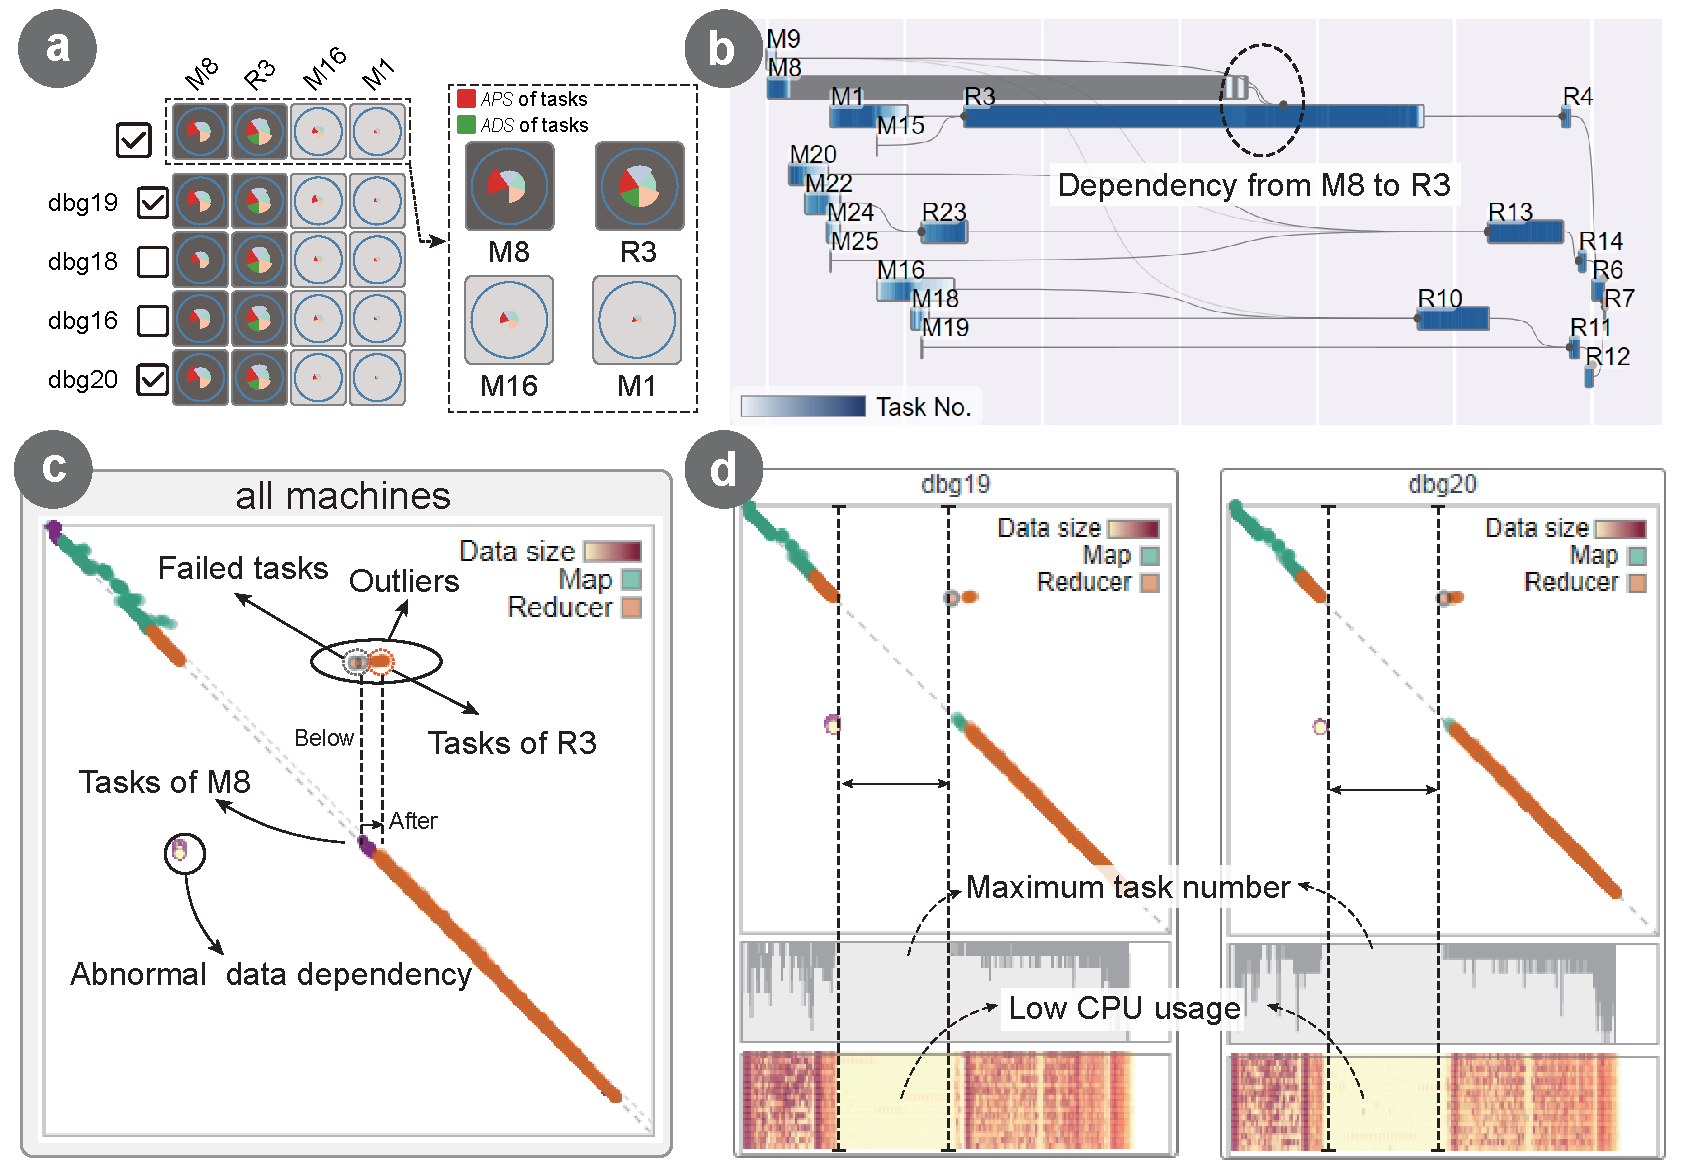
\includegraphics[width=0.46\textwidth]{figures/case_study/CaseStudy2SDS.pdf}  
	\vspace{-3mm}
	\caption{\qevis{} identifies system problem (task deadlock)} 
	\label{fig:casestudy2}
	\vspace{-5mm}
\end{figure}

\stitle{Step 1: observe abnormal jobs via \vtitle{performance matrix}}
As shown by the \textit{performance matrix} in \autoref{fig:casestudy2}(a), the anomaly scores of jobs R3 and M8 are significantly larger than the other jobs, especially the abnormal duration scores (i.e., red sectors). 
Moreover, the green sector (i.e., abnormal parallelism score) of job R3 is also very large.
Since job R3 is the downstream job of M8 as shown in the \textit{job view} in \autoref{fig:casestudy2}(b), 
we conjecture that there is a causal relation between the abnormal behaviors of jobs M8 and R3.


\stitle{Step 2: reveal abnormal data dependency via \vtitle{task view}}
We next perform fine-grained exploration on the tasks via the \vtitle{task view}.
There are several \textbf{outliers}, as highlighted in \autoref{fig:casestudy2}(c).
These outlier tasks can be classified into two categories: (i) failed tasks (the gray points), and (ii) long running tasks (highlighted in orange color).
Interestingly, several tasks of map job M8 are executed immediately after these failed tasks, and then the orange colored tasks of reducer job R3 are executed.
Visually, we can see there are several purple points (i.e., the tasks of job M8) vertically located below the gray points (i.e., failed tasks) and the orange points (i.e., tasks of job R3) are horizontally located after the purple points.
Thus, we confirm that there are abnormal data dependencies among the tasks of jobs M8 and R3, shown as the data dependency points in the left-bottom part of \autoref{fig:casestudy2}(c).


\stitle{Step 3: reason about the failed tasks via \vtitle{profiling view}}
As the \vtitle{profiling view} of the machine is aligned with \vtitle{task view} by time, 
we observe that both dbg19 and dbg20 run the maximum number of tasks during the execution period of these failed tasks, see the range between the two vertical dashed lines for dbg 19 and dbg20 in \autoref{fig:casestudy2}(d). 
However, the CPU utilization of two machines is very low in this period. 
This suggests that the containers of the two machines are fully occupied but no work is done, and thus there is a task deadlock.
In particular, the resource scheduler YARN assigns all containers of dbg19 and dbg20 to the tasks of job R3, and these tasks are waiting for the input data from the upstream tasks of job M8. But the upstream tasks cannot be executed as there are no idle containers, and thus the tasks of jobs M8 and R3 form a circular waiting.
The deadlock is resolved after killing several tasks of job R3, as depicted by the gray colored failed tasks in \autoref{fig:casestudy2}(c).

\qm{
	\stitle{Discussion} 
%	The deadlock appears when the computing resource is limited and too much containers are allocated by source manager(e.g., Yarn). \qevis{} can help analysts identify the deadlock cases with following features: by employing task level visualization with dependencies and properly aligning the timing information of tasks and system profiling.
%Deadlocks occur when computing resources are scarce and an excessive number of containers are allocated by the resource manager (e.g., Yarn). \qevis{} assist analysts to identify deadlock cases through the following features: task-level visualization incorporating dependencies and accurate alignment of timing information from tasks and system profiling. These capabilities enable analysts to gain insights into deadlock situations effectively.
%Deadlocks occur when computing resources are scarce and an excessive number of containers are allocated by the resource manager (e.g., Yarn). \qevis{} assist analysts to identify deadlock cases through the following features: task-level visualization incorporating dependencies and accurate alignment of timing information from tasks and system profiling. These capabilities enable analysts to gain insights into deadlock situations effectively.
%V1
%Deadlocks occur when there's a shortage of computing resources and the resource manager (e.g., Yarn) over-allocates containers. \qevis{} brings following features to address such scenarios: it represents task distribution, enabling users to swiftly identify critical tasks; it displays dependencies that indicate logical relationships among tasks; and it aligns system profiling with execution patterns to illustrate the interplay between resources and execution. The conventional approaches may struggle to manage this situation due to their lack of task oriented visaulization (both task and dependency) and task-system profiling alignment.
%V2
Deadlocks occur when there is a shortage of computing resources and suboptimal task scheduling by resource managers (e.g., Yarn). \qevis{} addresses this by offering following key features: task distribution for quick identification of critical tasks, dependency visualization for understanding logical task relationships and alignment of execution patterns with system profiling to show the interplay between resources and execution. The conventional approaches may struggle to manage this situation due to their lack of task oriented visualization (both task and dependency) and task-system profiling alignment.
}
\subsubsection{Identifying data problem}
We next analyze a query that runs daily for sales analysis, which takes 1200 seconds and is longer than before. 

\begin{figure}[t]
	\centering
	\small
	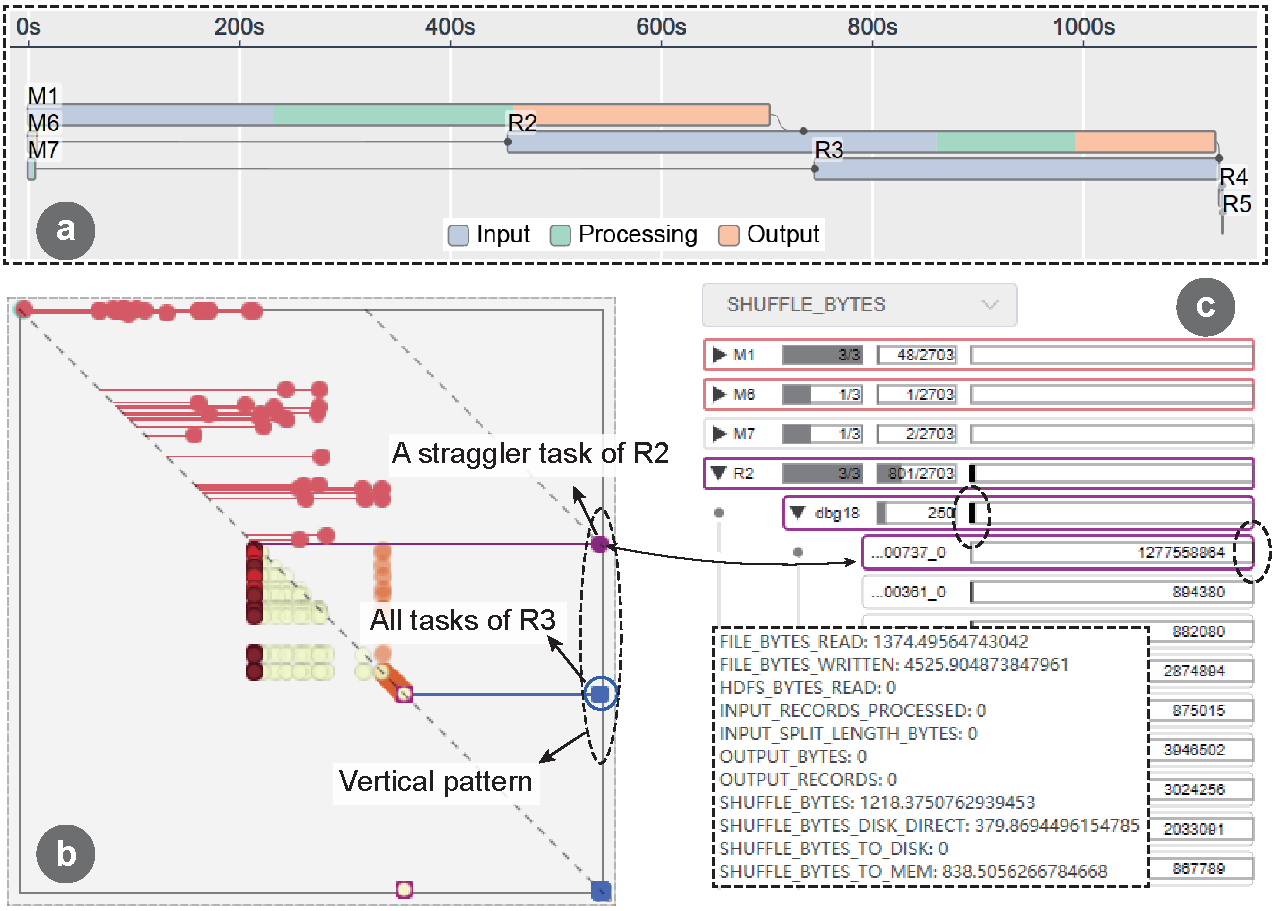
\includegraphics[width=0.46\textwidth]{figures/case_study/CaseStudy3SDS.pdf}
	\vspace{-2mm}
	\caption{\qevis{} detects data skew}
	\label{fig:casestudy3}
	\vspace{-5mm}
\end{figure}


\stitle{Step 1: identify performance bottleneck via \textit{job view}}
We inspect its \vtitle{job view} in \autoref{fig:casestudy3}(a) and observe that the input phase dominates the running time of job R3.
To find the reason for the long input time in job R3, we examine all its tasks via \vtitle{task view} in \autoref{fig:casestudy3}(b).


\stitle{Step 2: locate the straggler task via \textit{task view}}
We find that (i) all tasks of job R3 are concentrated in a small region, and (ii) there is a straggler task of job R2, which are highlighted in blue and purple circles in \autoref{fig:casestudy3}(b), respectively.
Moreover, there is a \textbf{vertical} execution pattern among the tasks of job R3 and the straggler task of job R2,
see the dashed eclipse, which suggests that the downstream tasks (of job R3) are waiting for the upstream task (of job R2).
%We next analyze the straggle task of job R2 via \vtitle{entity list}.

\stitle{Step 3: reason about the straggler task via \vtitle{entity list}}
By clicking the straggler task of job R2 in the \vtitle{task view}, the row of this task is automatically located and highlighted with a purple boundary in \autoref{fig:casestudy3}(c). 
We analyze its long running time by checking its processed data size, i.e., switching to ``SHUFFLE$\_$BYTES'' in the dropdown menu.
Surprisingly, the processed data volume of this straggler task is almost 1000 times of the other tasks in job R2, which indicates a severe data skew among the tasks.
Thus, the above unusually long running query is caused by data skew problem.

\qm{
	\stitle{Discussion} 
%	V1
%	In this case, multiple tasks exhibit abnormal execution behavior, but only one task, which suffers from data skewness, serves as the primary bottleneck for the entire execution process. Accurately identifying this specific bottleneck task necessitates the visualization of both tasks and their dependencies. This crucial visualization capability is provided exclusively by \qevis{}.
This case study highlights a scenario where a single task, experiencing data skewness, acts as the primary bottleneck in the execution process. Although multiple tasks exhibit abnormal execution behavior, correctly pinpointing this specific task is vital. This requires an intricate visualization of tasks along with their dependencies, a feature uniquely offered by \qevis{}.
}

%Through $\qevis$, we can conclude , then experienced engineers will try to alleviate it by re-configure the maximum number of task in Apache \hive{}. 

%\EVA{Can we show the optimization strategy?}



%\input{5.1_case}


%However, there is a straggler task, which incurs significantly long running time, 
%We find that the tasks of job R3 are all concentrated in a very small region (shown as \autoref{fig:casestudy3}(b2)) but an abnormal task runs significantly longer than the other tasks (shown as \autoref{fig:casestudy3}(b1)). 
%When hovering the mouse on task b1, we find that all tasks of R3 are colored blue, which means that task b1 was the provider for all tasks of R3 and the tasks of R3 are delayed because they are waiting for b1. After task b1 finishes, the entire query finishes almost immediately, suggesting that task b1 is the bottleneck of the query.



%one task of M24 runs for a long time on machine dbg19. Moreover, he also found a more obvious \textbf{dispersion pattern} in the \vtitle{task view} of dbg19 than the other machines, which indicates dbg19 is suffering from problem.







%The query is executed on a cluster with five machines (shown in \autoref{fig:teaser}(a)) and runs for about 623 seconds, which is much longer than usual. Thus, E1 used \qevis{} to find the reasons. 


%E1 started his exploration from the overview of query execution, i.e., \textit{job view} shown in \autoref{fig:teaser}(b). 
%phase 1 overview
%He found that job M1 had a significantly longer duration than the other jobs and had a long grey region indicating no tasks of M1 were executed during this period. Moreover, R2, a job consumed M1, finished quickly after M1 was completed, and the same applied to other reducer jobs (R3-6, 8, 10, 11) according to \autoref{fig:teaser}(b). 
%Thus, he inspected that M1 may be the performance bottleneck leading to the long execution time of this query.
% phase 2 detail view
%Then he hovered the mouse on M1 to highlight the associated tasks with purple color in the \vtitle{task view} shown as \autoref{fig:teaser}(d). 
%He observed that M1's tasks formed two groups far away from each other (\textbf{multi-cluster pattern}), as shown in the dashed ellipses in \autoref{fig:teaser}(d). 
%By checking the \vtitle{entity list} (shown as the rows with purple stroke in \autoref{fig:teaser}(e1)), he found that the tasks in the right-bottom corner were only executed on machine dbg18 since all the tasks executing on other machines finished much early.
%When observing the \vtitle{task view} of dbg18, he found dbg18 executed far fewer tasks than the other machines shown as \autoref{fig:teaser}(d1), which suggested that dbg18 may have internal problems. After checking the system log, he found that something was wrong with the network of dbg18, which caused the resource manager to allocate a small number of tasks to it and the late execution of these tasks. 

% phase 1, overview 
%Besides M1, he noticed that another Map job, M24, also had a long duration. By hovering the mouse on M24 to highlight its tasks, he found that none of them were executed on dbg18, and thus dbg18 was not the only performance bottleneck. 
% phase 2, detailed view
%In the \vtitle{task view}, he observed that one task of M24 runs for a long time on machine dbg19. Moreover, he also found a more obvious \textbf{dispersion pattern} in the \vtitle{task view} of dbg19 than the other machines, which indicates dbg19 is suffering from problem.
% phase 3, profiling view
%When exploring the system usage through \vtitle{profiling view}, he found that the CPU usage heatmap of dbg19 has large red regions, as shown in \autoref{fig:teaser}(f), indicating high CPU utilization. After a check, he found that several computation-intensive programs were also executed on dbg19 when running the query, resulting in resource contention.

%To address the identified problems, we remove machine dbg18 and kill the computation-intensive programs on machine dbg19. The query finishes within 200s this time. In the \textit{progress view}, we observe that the duration of both vertex M1 and M24 are much shorter than before, as shown in \autoref{fig:teaser}(B3). 
%We also find that all tasks are close to the diagonal line in the \textit{task distribution} in \autoref{fig:teaser}(D4)(\textbf{line parallel to diagonal} pattern in section~\ref{sec:taskdistribution}), indicating that they all have a short duration (thus no straggling task). 
%We also find that all tasks are close to the diagonal line in the \textit{task distribution} in \autoref{fig:teaser}(D4)(\textbf{line parallel to diagonal} pattern in section~\ref{sec:taskdistribution}), which is different from the previous \textbf{dispersion pattern}.





%\subsubsection{Reason task failure}




%The second query serves the purpose of generating a sales report sheet for the most recent two weeks. 
%It was run on a cluster with eight machines and was significantly slower than the last execution.
% \textcolor{red}{need to discribe the problem, to keep the same structure as 4.1}


%To further analyze the anomaly, we perform fine-grained exploration with the \vtitle{task view}.
%As dbg19 and dbg20 have significantly larger abnormal parallelism scores than the other machines (the red sector is larger), we inspect the \vtitle{task view} of all tasks (shown as \autoref{fig:casestudy2}(c)) and the \vtitle{task view} of these two machines (shown as \autoref{fig:casestudy2}(d)).
%From \autoref{fig:casestudy2}(c), we observe that most tasks are located close to the diagonal line, which is the \textbf{parallel pattern} (see Section~\ref{sec:task}) and indicates that they are  executed smoothly. However, there are several outliers in \autoref{fig:casestudy2}(c2), which is the \textbf{outlier pattern} and indicates that these tasks take much longer time than normal. Moreover, there are two failed tasks in these outliers (marked with grey boundaries). 
% \autoref{fig:casestudy2}(c) shows that most tasks were located close to the diagonal line (\textbf{parallel pattern}) while several outliers (\textbf{outlier pattern}) of R3 were far from the diagonal line, which is shown as \autoref{fig:casestudy2}(c2). 
% In addition, two of these tasks fail (marked with grey boundaries) and we want to know why. 

%\stitle{Step 3: }
%Now, we combine the \vtitle{task view} and \vtitle{profiling view} to find the causes of the failed tasks. 
%\vtitle{Task view} shows that the two failed tasks are executed on dbg19 and dbg20, respectively.
%As the \vtitle{profiling view} is aligned with \vtitle{task view} by time, we can observe that both dbg19 and dbg20 run the maximum number of tasks during the execution period of the two failed tasks (see the range marked by the two vertical dashed lines in \autoref{fig:casestudy2}(d1, d2)). 
%However, the CPU utilization of the two machines is low until the two tasks fail. This suggests that all containers of these two machines are occupied but these containers do not conduct work until the two tasks are killed. 
%Moreover, by hovering the mouse on the points in \autoref{fig:casestudy2}(c3), we observe that there are abnormal dependencies from tasks c1 to c2 in \autoref{fig:casestudy2}(c), indicating that job R3's task c2 is waiting for job M8's task c1.

%The observations above make us conjecture that the two tasks of R3 fail because of resource deadlock---job R3's task c2 waits for input from job M8's task c1 but all containers in dbg19 and dbg20 are occupied, and thus task c1 can not be scheduled, which blocks task c2 and prevents it from releasing the container. The system handles this deadlock by killing the two tasks of R3 on dbg19 and dbg20 to leave containers to execute M8's task c1, and R3's tasks finish quickly after receiving input data. 


%However, there is a straggler task, which incurs significantly long running time, 
%We find that the tasks of job R3 are all concentrated in a very small region (shown as \autoref{fig:casestudy3}(b2)) but an abnormal task runs significantly longer than the other tasks (shown as \autoref{fig:casestudy3}(b1)). 
%When hovering the mouse on task b1, we find that all tasks of R3 are colored blue, which means that task b1 was the provider for all tasks of R3 and the tasks of R3 are delayed because they are waiting for b1. After task b1 finishes, the entire query finishes almost immediately, suggesting that task b1 is the bottleneck of the query.



%one task of M24 runs for a long time on machine dbg19. Moreover, he also found a more obvious \textbf{dispersion pattern} in the \vtitle{task view} of dbg19 than the other machines, which indicates dbg19 is suffering from problem.







%The query is executed on a cluster with five machines (shown in \autoref{fig:teaser}(a)) and runs for about 623 seconds, which is much longer than usual. Thus, E1 used \qevis{} to find the reasons. 


%E1 started his exploration from the overview of query execution, i.e., \textit{job view} shown in \autoref{fig:teaser}(b). 
%phase 1 overview
%He found that job M1 had a significantly longer duration than the other jobs and had a long grey region indicating no tasks of M1 were executed during this period. Moreover, R2, a job consumed M1, finished quickly after M1 was completed, and the same applied to other reducer jobs (R3-6, 8, 10, 11) according to \autoref{fig:teaser}(b). 
%Thus, he inspected that M1 may be the performance bottleneck leading to the long execution time of this query.
% phase 2 detail view
%Then he hovered the mouse on M1 to highlight the associated tasks with purple color in the \vtitle{task view} shown as \autoref{fig:teaser}(d). 
%He observed that M1's tasks formed two groups far away from each other (\textbf{multi-cluster pattern}), as shown in the dashed ellipses in \autoref{fig:teaser}(d). 
%By checking the \vtitle{entity list} (shown as the rows with purple stroke in \autoref{fig:teaser}(e1)), he found that the tasks in the right-bottom corner were only executed on machine dbg18 since all the tasks executing on other machines finished much early.
%When observing the \vtitle{task view} of dbg18, he found dbg18 executed far fewer tasks than the other machines shown as \autoref{fig:teaser}(d1), which suggested that dbg18 may have internal problems. After checking the system log, he found that something was wrong with the network of dbg18, which caused the resource manager to allocate a small number of tasks to it and the late execution of these tasks. 

% phase 1, overview 
%Besides M1, he noticed that another Map job, M24, also had a long duration. By hovering the mouse on M24 to highlight its tasks, he found that none of them were executed on dbg18, and thus dbg18 was not the only performance bottleneck. 
% phase 2, detailed view
%In the \vtitle{task view}, he observed that one task of M24 runs for a long time on machine dbg19. Moreover, he also found a more obvious \textbf{dispersion pattern} in the \vtitle{task view} of dbg19 than the other machines, which indicates dbg19 is suffering from problem.
% phase 3, profiling view
%When exploring the system usage through \vtitle{profiling view}, he found that the CPU usage heatmap of dbg19 has large red regions, as shown in \autoref{fig:teaser}(f), indicating high CPU utilization. After a check, he found that several computation-intensive programs were also executed on dbg19 when running the query, resulting in resource contention.

%To address the identified problems, we remove machine dbg18 and kill the computation-intensive programs on machine dbg19. The query finishes within 200s this time. In the \textit{progress view}, we observe that the duration of both vertex M1 and M24 are much shorter than before, as shown in \autoref{fig:teaser}(B3). 
%We also find that all tasks are close to the diagonal line in the \textit{task distribution} in \autoref{fig:teaser}(D4)(\textbf{line parallel to diagonal} pattern in section~\ref{sec:taskdistribution}), indicating that they all have a short duration (thus no straggling task). 
%We also find that all tasks are close to the diagonal line in the \textit{task distribution} in \autoref{fig:teaser}(D4)(\textbf{line parallel to diagonal} pattern in section~\ref{sec:taskdistribution}), which is different from the previous \textbf{dispersion pattern}.





%\subsubsection{Reason task failure}




%The second query serves the purpose of generating a sales report sheet for the most recent two weeks. 
%It was run on a cluster with eight machines and was significantly slower than the last execution.
% \textcolor{red}{need to discribe the problem, to keep the same structure as 4.1}


%To further analyze the anomaly, we perform fine-grained exploration with the \vtitle{task view}.
%As dbg19 and dbg20 have significantly larger abnormal parallelism scores than the other machines (the red sector is larger), we inspect the \vtitle{task view} of all tasks (shown as \autoref{fig:casestudy2}(c)) and the \vtitle{task view} of these two machines (shown as \autoref{fig:casestudy2}(d)).
%From \autoref{fig:casestudy2}(c), we observe that most tasks are located close to the diagonal line, which is the \textbf{parallel pattern} (see Section~\ref{sec:task}) and indicates that they are  executed smoothly. However, there are several outliers in \autoref{fig:casestudy2}(c2), which is the \textbf{outlier pattern} and indicates that these tasks take much longer time than normal. Moreover, there are two failed tasks in these outliers (marked with grey boundaries). 
% \autoref{fig:casestudy2}(c) shows that most tasks were located close to the diagonal line (\textbf{parallel pattern}) while several outliers (\textbf{outlier pattern}) of R3 were far from the diagonal line, which is shown as \autoref{fig:casestudy2}(c2). 
% In addition, two of these tasks fail (marked with grey boundaries) and we want to know why. 

%\stitle{Step 3: }
%Now, we combine the \vtitle{task view} and \vtitle{profiling view} to find the causes of the failed tasks. 
%\vtitle{Task view} shows that the two failed tasks are executed on dbg19 and dbg20, respectively.
%As the \vtitle{profiling view} is aligned with \vtitle{task view} by time, we can observe that both dbg19 and dbg20 run the maximum number of tasks during the execution period of the two failed tasks (see the range marked by the two vertical dashed lines in \autoref{fig:casestudy2}(d1, d2)). 
%However, the CPU utilization of the two machines is low until the two tasks fail. This suggests that all containers of these two machines are occupied but these containers do not conduct work until the two tasks are killed. 
%Moreover, by hovering the mouse on the points in \autoref{fig:casestudy2}(c3), we observe that there are abnormal dependencies from tasks c1 to c2 in \autoref{fig:casestudy2}(c), indicating that job R3's task c2 is waiting for job M8's task c1.

%The observations above make us conjecture that the two tasks of R3 fail because of resource deadlock---job R3's task c2 waits for input from job M8's task c1 but all containers in dbg19 and dbg20 are occupied, and thus task c1 can not be scheduled, which blocks task c2 and prevents it from releasing the container. The system handles this deadlock by killing the two tasks of R3 on dbg19 and dbg20 to leave containers to execute M8's task c1, and R3's tasks finish quickly after receiving input data. 


%However, there is a straggler task, which incurs significantly long running time, 
%We find that the tasks of job R3 are all concentrated in a very small region (shown as \autoref{fig:casestudy3}(b2)) but an abnormal task runs significantly longer than the other tasks (shown as \autoref{fig:casestudy3}(b1)). 
%When hovering the mouse on task b1, we find that all tasks of R3 are colored blue, which means that task b1 was the provider for all tasks of R3 and the tasks of R3 are delayed because they are waiting for b1. After task b1 finishes, the entire query finishes almost immediately, suggesting that task b1 is the bottleneck of the query.



%one task of M24 runs for a long time on machine dbg19. Moreover, he also found a more obvious \textbf{dispersion pattern} in the \vtitle{task view} of dbg19 than the other machines, which indicates dbg19 is suffering from problem.







%The query is executed on a cluster with five machines (shown in \autoref{fig:teaser}(a)) and runs for about 623 seconds, which is much longer than usual. Thus, E1 used \qevis{} to find the reasons. 


%E1 started his exploration from the overview of query execution, i.e., \textit{job view} shown in \autoref{fig:teaser}(b). 
%phase 1 overview
%He found that job M1 had a significantly longer duration than the other jobs and had a long grey region indicating no tasks of M1 were executed during this period. Moreover, R2, a job consumed M1, finished quickly after M1 was completed, and the same applied to other reducer jobs (R3-6, 8, 10, 11) according to \autoref{fig:teaser}(b). 
%Thus, he inspected that M1 may be the performance bottleneck leading to the long execution time of this query.
% phase 2 detail view
%Then he hovered the mouse on M1 to highlight the associated tasks with purple color in the \vtitle{task view} shown as \autoref{fig:teaser}(d). 
%He observed that M1's tasks formed two groups far away from each other (\textbf{multi-cluster pattern}), as shown in the dashed ellipses in \autoref{fig:teaser}(d). 
%By checking the \vtitle{entity list} (shown as the rows with purple stroke in \autoref{fig:teaser}(e1)), he found that the tasks in the right-bottom corner were only executed on machine dbg18 since all the tasks executing on other machines finished much early.
%When observing the \vtitle{task view} of dbg18, he found dbg18 executed far fewer tasks than the other machines shown as \autoref{fig:teaser}(d1), which suggested that dbg18 may have internal problems. After checking the system log, he found that something was wrong with the network of dbg18, which caused the resource manager to allocate a small number of tasks to it and the late execution of these tasks. 

% phase 1, overview 
%Besides M1, he noticed that another Map job, M24, also had a long duration. By hovering the mouse on M24 to highlight its tasks, he found that none of them were executed on dbg18, and thus dbg18 was not the only performance bottleneck. 
% phase 2, detailed view
%In the \vtitle{task view}, he observed that one task of M24 runs for a long time on machine dbg19. Moreover, he also found a more obvious \textbf{dispersion pattern} in the \vtitle{task view} of dbg19 than the other machines, which indicates dbg19 is suffering from problem.
% phase 3, profiling view
%When exploring the system usage through \vtitle{profiling view}, he found that the CPU usage heatmap of dbg19 has large red regions, as shown in \autoref{fig:teaser}(f), indicating high CPU utilization. After a check, he found that several computation-intensive programs were also executed on dbg19 when running the query, resulting in resource contention.

%To address the identified problems, we remove machine dbg18 and kill the computation-intensive programs on machine dbg19. The query finishes within 200s this time. In the \textit{progress view}, we observe that the duration of both vertex M1 and M24 are much shorter than before, as shown in \autoref{fig:teaser}(B3). 
%We also find that all tasks are close to the diagonal line in the \textit{task distribution} in \autoref{fig:teaser}(D4)(\textbf{line parallel to diagonal} pattern in section~\ref{sec:taskdistribution}), indicating that they all have a short duration (thus no straggling task). 
%We also find that all tasks are close to the diagonal line in the \textit{task distribution} in \autoref{fig:teaser}(D4)(\textbf{line parallel to diagonal} pattern in section~\ref{sec:taskdistribution}), which is different from the previous \textbf{dispersion pattern}.





%\subsubsection{Reason task failure}




%The second query serves the purpose of generating a sales report sheet for the most recent two weeks. 
%It was run on a cluster with eight machines and was significantly slower than the last execution.
% \textcolor{red}{need to discribe the problem, to keep the same structure as 4.1}


%To further analyze the anomaly, we perform fine-grained exploration with the \vtitle{task view}.
%As dbg19 and dbg20 have significantly larger abnormal parallelism scores than the other machines (the red sector is larger), we inspect the \vtitle{task view} of all tasks (shown as \autoref{fig:casestudy2}(c)) and the \vtitle{task view} of these two machines (shown as \autoref{fig:casestudy2}(d)).
%From \autoref{fig:casestudy2}(c), we observe that most tasks are located close to the diagonal line, which is the \textbf{parallel pattern} (see Section~\ref{sec:task}) and indicates that they are  executed smoothly. However, there are several outliers in \autoref{fig:casestudy2}(c2), which is the \textbf{outlier pattern} and indicates that these tasks take much longer time than normal. Moreover, there are two failed tasks in these outliers (marked with grey boundaries). 
% \autoref{fig:casestudy2}(c) shows that most tasks were located close to the diagonal line (\textbf{parallel pattern}) while several outliers (\textbf{outlier pattern}) of R3 were far from the diagonal line, which is shown as \autoref{fig:casestudy2}(c2). 
% In addition, two of these tasks fail (marked with grey boundaries) and we want to know why. 

%\stitle{Step 3: }
%Now, we combine the \vtitle{task view} and \vtitle{profiling view} to find the causes of the failed tasks. 
%\vtitle{Task view} shows that the two failed tasks are executed on dbg19 and dbg20, respectively.
%As the \vtitle{profiling view} is aligned with \vtitle{task view} by time, we can observe that both dbg19 and dbg20 run the maximum number of tasks during the execution period of the two failed tasks (see the range marked by the two vertical dashed lines in \autoref{fig:casestudy2}(d1, d2)). 
%However, the CPU utilization of the two machines is low until the two tasks fail. This suggests that all containers of these two machines are occupied but these containers do not conduct work until the two tasks are killed. 
%Moreover, by hovering the mouse on the points in \autoref{fig:casestudy2}(c3), we observe that there are abnormal dependencies from tasks c1 to c2 in \autoref{fig:casestudy2}(c), indicating that job R3's task c2 is waiting for job M8's task c1.

%The observations above make us conjecture that the two tasks of R3 fail because of resource deadlock---job R3's task c2 waits for input from job M8's task c1 but all containers in dbg19 and dbg20 are occupied, and thus task c1 can not be scheduled, which blocks task c2 and prevents it from releasing the container. The system handles this deadlock by killing the two tasks of R3 on dbg19 and dbg20 to leave containers to execute M8's task c1, and R3's tasks finish quickly after receiving input data. 


%However, there is a straggler task, which incurs significantly long running time, 
%We find that the tasks of job R3 are all concentrated in a very small region (shown as \autoref{fig:casestudy3}(b2)) but an abnormal task runs significantly longer than the other tasks (shown as \autoref{fig:casestudy3}(b1)). 
%When hovering the mouse on task b1, we find that all tasks of R3 are colored blue, which means that task b1 was the provider for all tasks of R3 and the tasks of R3 are delayed because they are waiting for b1. After task b1 finishes, the entire query finishes almost immediately, suggesting that task b1 is the bottleneck of the query.



%one task of M24 runs for a long time on machine dbg19. Moreover, he also found a more obvious \textbf{dispersion pattern} in the \vtitle{task view} of dbg19 than the other machines, which indicates dbg19 is suffering from problem.







%The query is executed on a cluster with five machines (shown in \autoref{fig:teaser}(a)) and runs for about 623 seconds, which is much longer than usual. Thus, E1 used \qevis{} to find the reasons. 


%E1 started his exploration from the overview of query execution, i.e., \textit{job view} shown in \autoref{fig:teaser}(b). 
%phase 1 overview
%He found that job M1 had a significantly longer duration than the other jobs and had a long grey region indicating no tasks of M1 were executed during this period. Moreover, R2, a job consumed M1, finished quickly after M1 was completed, and the same applied to other reducer jobs (R3-6, 8, 10, 11) according to \autoref{fig:teaser}(b). 
%Thus, he inspected that M1 may be the performance bottleneck leading to the long execution time of this query.
% phase 2 detail view
%Then he hovered the mouse on M1 to highlight the associated tasks with purple color in the \vtitle{task view} shown as \autoref{fig:teaser}(d). 
%He observed that M1's tasks formed two groups far away from each other (\textbf{multi-cluster pattern}), as shown in the dashed ellipses in \autoref{fig:teaser}(d). 
%By checking the \vtitle{entity list} (shown as the rows with purple stroke in \autoref{fig:teaser}(e1)), he found that the tasks in the right-bottom corner were only executed on machine dbg18 since all the tasks executing on other machines finished much early.
%When observing the \vtitle{task view} of dbg18, he found dbg18 executed far fewer tasks than the other machines shown as \autoref{fig:teaser}(d1), which suggested that dbg18 may have internal problems. After checking the system log, he found that something was wrong with the network of dbg18, which caused the resource manager to allocate a small number of tasks to it and the late execution of these tasks. 

% phase 1, overview 
%Besides M1, he noticed that another Map job, M24, also had a long duration. By hovering the mouse on M24 to highlight its tasks, he found that none of them were executed on dbg18, and thus dbg18 was not the only performance bottleneck. 
% phase 2, detailed view
%In the \vtitle{task view}, he observed that one task of M24 runs for a long time on machine dbg19. Moreover, he also found a more obvious \textbf{dispersion pattern} in the \vtitle{task view} of dbg19 than the other machines, which indicates dbg19 is suffering from problem.
% phase 3, profiling view
%When exploring the system usage through \vtitle{profiling view}, he found that the CPU usage heatmap of dbg19 has large red regions, as shown in \autoref{fig:teaser}(f), indicating high CPU utilization. After a check, he found that several computation-intensive programs were also executed on dbg19 when running the query, resulting in resource contention.

%To address the identified problems, we remove machine dbg18 and kill the computation-intensive programs on machine dbg19. The query finishes within 200s this time. In the \textit{progress view}, we observe that the duration of both vertex M1 and M24 are much shorter than before, as shown in \autoref{fig:teaser}(B3). 
%We also find that all tasks are close to the diagonal line in the \textit{task distribution} in \autoref{fig:teaser}(D4)(\textbf{line parallel to diagonal} pattern in section~\ref{sec:taskdistribution}), indicating that they all have a short duration (thus no straggling task). 
%We also find that all tasks are close to the diagonal line in the \textit{task distribution} in \autoref{fig:teaser}(D4)(\textbf{line parallel to diagonal} pattern in section~\ref{sec:taskdistribution}), which is different from the previous \textbf{dispersion pattern}.





%\subsubsection{Reason task failure}




%The second query serves the purpose of generating a sales report sheet for the most recent two weeks. 
%It was run on a cluster with eight machines and was significantly slower than the last execution.
% \textcolor{red}{need to discribe the problem, to keep the same structure as 4.1}


%To further analyze the anomaly, we perform fine-grained exploration with the \vtitle{task view}.
%As dbg19 and dbg20 have significantly larger abnormal parallelism scores than the other machines (the red sector is larger), we inspect the \vtitle{task view} of all tasks (shown as \autoref{fig:casestudy2}(c)) and the \vtitle{task view} of these two machines (shown as \autoref{fig:casestudy2}(d)).
%From \autoref{fig:casestudy2}(c), we observe that most tasks are located close to the diagonal line, which is the \textbf{parallel pattern} (see Section~\ref{sec:task}) and indicates that they are  executed smoothly. However, there are several outliers in \autoref{fig:casestudy2}(c2), which is the \textbf{outlier pattern} and indicates that these tasks take much longer time than normal. Moreover, there are two failed tasks in these outliers (marked with grey boundaries). 
% \autoref{fig:casestudy2}(c) shows that most tasks were located close to the diagonal line (\textbf{parallel pattern}) while several outliers (\textbf{outlier pattern}) of R3 were far from the diagonal line, which is shown as \autoref{fig:casestudy2}(c2). 
% In addition, two of these tasks fail (marked with grey boundaries) and we want to know why. 

%\stitle{Step 3: }
%Now, we combine the \vtitle{task view} and \vtitle{profiling view} to find the causes of the failed tasks. 
%\vtitle{Task view} shows that the two failed tasks are executed on dbg19 and dbg20, respectively.
%As the \vtitle{profiling view} is aligned with \vtitle{task view} by time, we can observe that both dbg19 and dbg20 run the maximum number of tasks during the execution period of the two failed tasks (see the range marked by the two vertical dashed lines in \autoref{fig:casestudy2}(d1, d2)). 
%However, the CPU utilization of the two machines is low until the two tasks fail. This suggests that all containers of these two machines are occupied but these containers do not conduct work until the two tasks are killed. 
%Moreover, by hovering the mouse on the points in \autoref{fig:casestudy2}(c3), we observe that there are abnormal dependencies from tasks c1 to c2 in \autoref{fig:casestudy2}(c), indicating that job R3's task c2 is waiting for job M8's task c1.

%The observations above make us conjecture that the two tasks of R3 fail because of resource deadlock---job R3's task c2 waits for input from job M8's task c1 but all containers in dbg19 and dbg20 are occupied, and thus task c1 can not be scheduled, which blocks task c2 and prevents it from releasing the container. The system handles this deadlock by killing the two tasks of R3 on dbg19 and dbg20 to leave containers to execute M8's task c1, and R3's tasks finish quickly after receiving input data. 